% This is the Reed College LaTeX thesis template. Most of the work
% template. Later comments etc. by Ben Salzberg (BTS). Additional
% restructuring and APA support by Jess Youngberg (JY).
% Your comments and suggestions are more than welcome; please email
% them to cus@reed.edu
%
% See http://web.reed.edu/cis/help/latex.html for help. There are a
% great bunch of help pages there, with notes on
% getting started, bibtex, etc. Go there and read it if you're not
% already familiar with LaTeX.
%
% Any line that starts with a percent symbol is a comment.
% They won't show up in the document, and are useful for notes
% to yourself and explaining commands.
% Commenting also removes a line from the document;
% very handy for troubleshooting problems. -BTS

% As far as I know, this follows the requirements laid out in
% the 2002-2003 Senior Handbook. Ask a librarian to check the
% document before binding. -SN

%%
%% Preamble
%%
% \documentclass{<something>} must begin each LaTeX document
\documentclass[12pt,twoside]{reedthesis}
% Packages are extensions to the basic LaTeX functions. Whatever you
% want to typeset, there is probably a package out there for it.
% Chemistry (chemtex), screenplays, you name it.
% Check out CTAN to see: http://www.ctan.org/
%%
\usepackage{graphicx,latexsym}
\usepackage{amsmath}
\usepackage{amssymb,amsthm}
\usepackage{longtable,booktabs,setspace}
\usepackage{chemarr} %% Useful for one reaction arrow, useless if you're not a chem major
\usepackage{rotating}

% Modified by CII
\usepackage[hyphens]{url}
\usepackage{hyperref}
\usepackage{lmodern}

% Added by CII (Thanks, Hadley!)
% Use ref for internal links
\renewcommand{\hyperref}[2][???]{\autoref{#1}}
\def\chapterautorefname{Chapter}
\def\sectionautorefname{Section}
\def\subsectionautorefname{Subsection}

\usepackage{caption}
\captionsetup{width=5in}

% \usepackage{times} % other fonts are available like times, bookman, charter, palatino

\title{A Random Forest Model for Computer-Assisted Activity-Recognition}
\author{Elizabeth S. Ash}
% The month and year that you submit your FINAL draft TO THE LIBRARY (May or December)
\date{May 2016}
\division{Mathematics}
\advisor{Dr.~Homer White}
%If you have two advisors for some reason, you can use the following
\altadvisor{Dr.~David Bowman}
%%% Remember to use the correct department!
\department{Mathematics}
% if you're writing a thesis in an interdisciplinary major,
% uncomment the line below and change the text as appropriate.
% check the Senior Handbook if unsure.
%\thedivisionof{The Established Interdisciplinary Committee for}
% if you want the approval page to say "Approved for the Committee",
% uncomment the next line
%\approvedforthe{Committee}

% Below added by CII

%%% Copied from knitr
%% maxwidth is the original width if it's less than linewidth
%% otherwise use linewidth (to make sure the graphics do not exceed the margin)
\makeatletter
\def\maxwidth{ %
  \ifdim\Gin@nat@width>\linewidth
    \linewidth
  \else
    \Gin@nat@width
  \fi
}
\makeatother

\renewcommand{\contentsname}{Table of Contents}

\setlength{\parskip}{0pt}

  %\setlength{\parskip}{\baselineskip}
  \usepackage[parfill]{parskip}

\providecommand{\tightlist}{%
  \setlength{\itemsep}{0pt}\setlength{\parskip}{0pt}}

\Acknowledgements{

}

\Dedication{

}

\Preface{

}

\Abstract{
We use predictive models to create a statistical model of future
behavior. In particular, we examine how well a random forest predictive
model would predict the classification of a new lift by the same
experimental subjects. We separate the data into training and test sets
using the variable \texttt{num\_window} to ensure that a single lift is
not in both sets. We find that a random forest model can accurately and
`honestly' predict the classifications of the weight lift type performed
by the experimental subjects.
}


%%
%% End Preamble
%%
%

\begin{document}

      \maketitle
  
  \frontmatter % this stuff will be roman-numbered
  \pagestyle{empty} % this removes page numbers from the frontmatter

  
  
  % Add table of abbreviations?

      \hypersetup{linkcolor=black}
    \setcounter{tocdepth}{4}
    \tableofcontents
  
      \listoftables
  
      \listoffigures
  
      \begin{abstract}
      We use predictive models to create a statistical model of future
      behavior. In particular, we examine how well a random forest predictive
      model would predict the classification of a new lift by the same
      experimental subjects. We separate the data into training and test sets
      using the variable \texttt{num\_window} to ensure that a single lift is
      not in both sets. We find that a random forest model can accurately and
      `honestly' predict the classifications of the weight lift type performed
      by the experimental subjects.
    \end{abstract}
  
  
  \mainmatter % here the regular arabic numbering starts
  \pagestyle{fancyplain} % turns page numbering back on

  \chapter*{Introduction and Overview}\label{introduction-and-overview}
  \addcontentsline{toc}{chapter}{Introduction and Overview}
  
  Predictive modeling is a process used to create a statistical model of
  future behavior. A predictive model is made up of a number of
  \textbf{predictors}, which are variable factors that are likely to
  influence future behaviors or results. Gareth James, Daniela Witten,
  Trevor Hastie and Robert Tibshirani give an example in their book
  \emph{An Introduction to Statistical Learning with Applications in R} to
  briefly introduce the topic of predictor variables:
  
  \begin{quote}
  Suppose we are statistical consultants hired by a company to provided
  advice on how to improve sales of a particular product\ldots{}It is not
  possible for our client to directly increase the sales of the product.
  On the other hand, they can control the advertising expenditure in each
  of the three media {[}TV, radio and newspapers{]}. Therefore, if we
  determine that there is an association between advertising and sales,
  then we can instruct our client to adjust advertising budgets, thereby
  indirectly increasing sales. In other words, our goal is to develop an
  accurate model that can be used to predict sales on the basis of the
  three media budgets (James, 2013).
  \end{quote}
  
  In this example, James, et al. use media budgets for TV, radio, and
  newspapers as the predictor variables and the sales of a particular
  product is the response variable. Using predictive modeling, the company
  can then use the predictor variables to predict the sales outcomes of
  the particular product.
  
  In predictive modeling, data is collected for the relevant predictors, a
  statistical model is formulated, predictions are made, and the model is
  revised as additional data becomes available. My research project deals
  with predictive models and applications of such modeling.
  
  An example of an application of predictive modeling is activity
  recognition. Activity recognition is an increasingly important
  technology because it can be applied to many real-life problems such as,
  home-based proactive and preventive healthcare applications. It can also
  be applied in learning environments, security systems, and a variety of
  human-computer interfaces. The goal of activity recognition is to
  recognize common human activities in real-life settings.
  
  One real-life setting example of activity recogniton is physical
  activity, which is one of the most important things that can be done for
  overall health. It can help control weight, lower risk for heart
  disease, strengthen bones and muscles, and increase chances of longer
  life. However, if the activity is performed incorrectly, there is a
  greater risk of injury, which is counterproductive. To benefit most from
  a fitness routine, the activity should be performed as accurately as
  possible. Some people can go to a gym and work with a certified trainer,
  but many people cannot or will not work with a personal trainer. These
  people may be doing the correct exercise motion, but there is no way to
  really know unless they are taught the correct motion by a professional.
  Using other physical activities as predictor variables, a predictive
  model could be made and used to help determine if the exercise motion is
  being executed properly.
  
  In the case of my research project, I want to see if a predictive model
  can be made to recognize certain weight lift motions. If a predictor
  model could be made, then the model could be integrated into the weight
  lift equipment and used to determine if the lift was done correctly or
  incorrectly. This model could be integrated with other technologies and
  be used to help reinforce the correct weight lift motion by commending
  the user for a correct movement or making a comment when the user made
  an incorrect movement. For example, I am trying to perform the lift
  motion from the study correctly, but I am actually performing an error.
  If my predictive model is good enough (based on the measurements from
  the sensors, the model can accurately predict in which class my lift
  belongs), then my armband could beep, notifying me of my error.
  
  \section{Background on Data Used}\label{background-on-data-used}
  
  The article \emph{Qualitative Activity Recognition of Weight Lifting
  Exercises} describes a study presented by Eduardo Velloso, Andreas
  Bulling, Hans Gellersen, Wallace Ugulino, and Hugo Fuks. Among other
  goals, the researchers wanted to provide feedback to weight lifters
  using qualitative activity recognition. The study involved six male
  subjects, all in their twenties and with little weight lifting
  experience. The subjects were taught how to lift a dumb-bell correctly
  and were also taught how to perform the same movement in four incorrect
  ways. The Unilateral Dumbbell Bicep Curl was the lift that was taught to
  the subjects. The five categories of lift data collected were:
  
  \begin{verbatim}
  * Class A: correct lift movement
  * Class B: throwing the elbows to the front
  * Class C: lifting the dumbbell only halfway
  * Class D: lowering the dumbbell only halfway
  * Class E: throwing the hips to the front
  \end{verbatim}
  
  The subjects repeated each lift ten times and during each lift the
  researchers recorded a number of inertial measurements from sensors in
  the users' glove, armband, lumbar belt, and dumbbell (these are pieces
  of equipment that are commonly used by weight lifters). These
  measurements make up the predictors that the researchers used when
  determing a correct or incorrect lift. The sensors recorded several data
  points throughout the lifting motion and the final data set includes 160
  variables. Some of the variables included are: user\_name, num\_window,
  yaw\_belt, pitch\_belt, and total\_accel\_belt.
  
  The aim of this report is to build a predictive model that can be used
  in realistic circumstances built on the data from the Velloso et al
  study.
  
  \chapter{Methods}\label{rmd-basics}
  
  \section{Background on Methods Used}\label{background-on-methods-used}
  
  The method of model making that will be used in this report is random
  forest. A more detailed discussion of the random forest method will
  follow. However, there are some concepts and definitions that need to be
  addressed before the random forest method can be fully understood. The
  first important concept is a classification tree, which is used in the
  construction of a random forest model.
  
  \section{Classification Trees}\label{classification-trees}
  
  Classification trees are a tree-based model and are used to predict a
  qualitative response. The variables that go into these classification
  trees can be numerical or categorical. We predict that ``each
  observation belongs to the most commonly occuring class (or category) of
  training observations in the region to which it belongs'' (James, 2013).
  They are useful because they provide predictors in situations where
  there are many variables that interact in complicated, non-linear ways.
  In interpreting these classification trees, we are often ``interested in
  both the class prediction corresponding to a particular terminal node
  region, and in the class proportions among the training observations
  that fall into that region'' (James, 2013).
  
  So, in simpler terms, a classification tree consists of a set of
  true/false decision rules. It is kind of like a game of 20 questions,
  where we ask different questions based on the answers to previous
  questions, and then at the end we make a guess based on all the answers.
  We can visualize a decision tree as a set of nodes (corresponding to
  true/false questions), each of which has two branches depending on the
  answer to the question. Unlike real trees, we usually draw them with
  their ``root'' at the top, and the ``leaves'' at the bottom. In order to
  make predictions with the tree, we start at the top (the ``root'' node),
  and ask questions, traveling left or right in the tree based on what the
  answer is (left for true and right for false). At each step, we reach a
  new node, with a new question. Once we reach the bottom (a leaf node),
  we make a prediction based on the set of answers, just like 20
  questions. But unlike 20 questions, the number of questions in a
  decision tree is not always 20, but can vary (Corso, 2013).
  
  Shall we look at an example of a classification tree?
  
  We are using a data set from a survey taken in the MAT 111 class
  (Elementary Probability and Statistics) at Georgetown College. This data
  set has 71 rows and 12 variables. The survey includes variables such as
  sex, height, GPA, sleep, and the fastest speed ever driven. The names of
  some of the variables may seem a little odd, such as weight\_feel,
  love\_first, and extra\_life. The weight\_feel variable is how the
  participant feels about their weight. They could have answered
  underweight (``a''), about right (``b''), or overweight (``c''). The
  love\_feel variable is whether or not the participant believes in love
  at first sight and the extra\_life variable is whether or not the
  participant believes in extraterrestrial life. The seat variable is
  where the participant sits in a classroom. The letter ``a'' corresponds
  to sitting in the front, ``b'' corresponds sitting in the middle rows,
  and ``c'' corresponds to sitting in the back rows.
  
  \subsection{An Extended Example of a Classification
  Tree}\label{an-extended-example-of-a-classification-tree}
  
  This tree is used to predict the sex of an individual based on the
  variables of fastest speed ever driven, GPA, height, the amount of sleep
  the participant got the night before, how the participant feels about
  their weight, and if the participant believes in love at first sight. R
  code is not only a great tool for making classification trees, it can
  also print a readable version of classification trees. Below is an easy
  to understand schematic of a classification tree.
  
  \begin{figure}
  
  {\centering 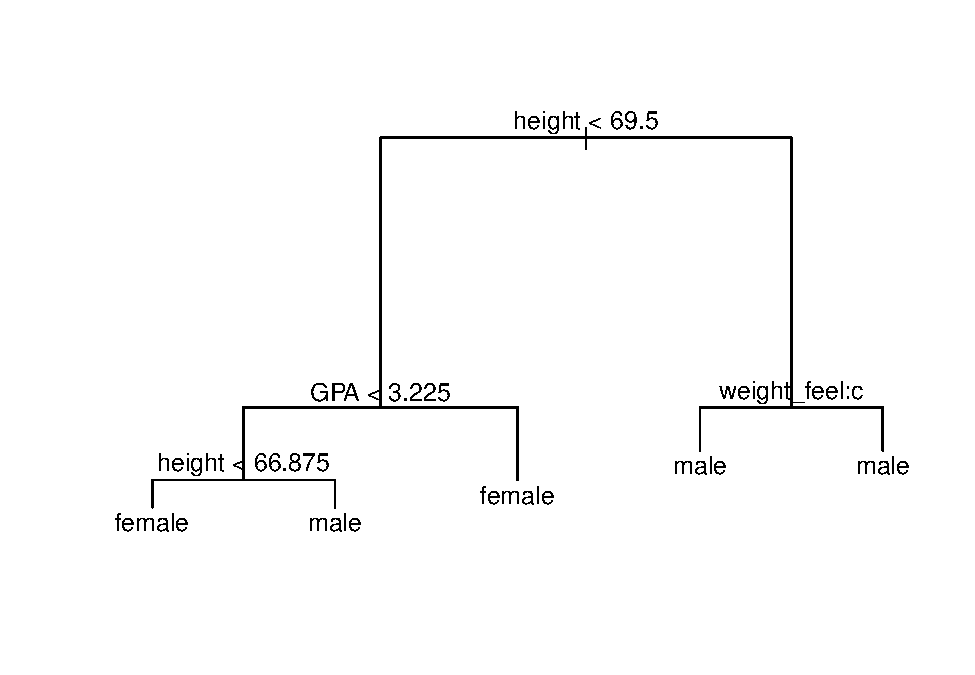
\includegraphics{A_Random_Forest_Model_for_Computer-Assisted_Activity-Recognition_files/figure-latex/unnamed-chunk-4-1} 
  
  }
  
  \caption[Classification tree to predict sex in m111survey data]{Classification tree to predict sex in m111survey data}\label{fig:unnamed-chunk-4}
  \end{figure}
  
  All classification trees have nodes. The top node is referred to as the
  \emph{root} node. Nodes can either split into two \emph{daughter} nodes
  (or leaves) or they can stop splitting. A node that does not split any
  further is known as a \emph{terminal} node. In this tree example, the
  majority sex in each terminal node is given under the node. This tree
  can be used to predict if a new individual is male or female. All we
  have to do is ask YES or NO questions and follow the nodes to a terminal
  node.
  
  So, by looking at this tree, we can see that the first splits is set
  when height is less than 69.5 inches. If the height of an observation is
  less than 69.5 inches they are put into the left region and those with a
  height equal to or above 69.5 inches are put into the right region.
  Those in the left hand region are divided by GPA. If the GPA is greater
  than or equal to 3.225, the prediction is female. If the GPA is less
  than 3.225, then a further division by height is made. If the height is
  less than 66.875 inches, then female is predicted. Otherwise, the sex is
  predicted as male. Those in the right region are divided by how they
  feel about their weight. Notice that the division is by
  ``weight\_feel:c''. This means that the left region feel underweight or
  about right and the right region feel overweight. Instead of using the
  full name of the variable, this tree made shorter version. The letter
  ``a'' corresponds to feeling underweight, the letter ``b'' corresponds
  to feeling about right, and the letter ``c'' corresponds to feeling
  overweight. Looking at the two terminal nodes, it appears that it
  doesn't matter how they feel about their weight; the prediction will
  still be male.
  
  Below is the same classification tree, but with more details:
  
  \begin{verbatim}
  node), split, n, deviance, yval, (yprob)
        * denotes terminal node
  
  1) root 70 96.120 female ( 0.5571 0.4429 )  
    2) height < 69.5 42 34.450 female ( 0.8571 0.1429 )  
      4) GPA < 3.225 18 22.910 female ( 0.6667 0.3333 )  
        8) height < 66.875 9  6.279 female ( 0.8889 0.1111 ) *
        9) height > 66.875 9 12.370 male ( 0.4444 0.5556 ) *
      5) GPA > 3.225 24  0.000 female ( 1.0000 0.0000 ) *
    3) height > 69.5 28 19.070 male ( 0.1071 0.8929 )  
      6) weight_feel: 3_overweight 10 12.220 male ( 0.3000 0.7000 ) *
      7) weight_feel: 1_underweight,2_about_right 18  0.000 male ( 0.0000 1.0000 ) *
  \end{verbatim}
  
  This printout actually gives us quite a bit of information about the
  classification tree. First, the node numbers are labeled. So the root
  node is number 1 and the daughter nodes are numbers 2 and 3. Second, the
  variable by which the split was made is given. For example, the root
  node is split based on height. With daughter node 2, any height less
  than 69.5 inches would be placed in that node. And for daughter node 3,
  any height greater than 69.5 inches would be placed in that node. Third,
  the number of cases that reach the node is given. For example, there are
  70 observations in the root node. {[}As a note, classification trees do
  not like missing data, so one row from the original data set was removed
  to avoid any missing values.{]} After the root node is split, 42
  observations are found in daughter node 2 and 28 observations are found
  in daughter node 3. The sum of the two observations is 70. The fourth
  piece of information given by the printout is deviance, which is an
  assessment of goodness of fit (we will go into this a litte later). The
  fifth piece of information in the prinout is the yval, which is the
  majority value for the node. This would be predicted for that node. For
  example, if the tree was forced to make a prediction about the sex at
  node 4, the tree would predict that the individual would be female. The
  final piece of information from the printout is the yprob, which gives
  the probabilities of the variables being predicted. In node 4, (0.6667
  0.3333) is given. This means that 66.67\% of the objects in the node are
  female and 33.33\% of the objects are male. The yval proportions can
  also be used to assign a probability to the prediction of a new person.
  For example, if we were to try to predict the sex of a new individual
  (using this classification tree) and the tree had to make a guess at
  node 4, the new individual would be predicted to be female. Female is
  the majority sex in this node, which is why a female prediction would be
  made. In addition, the yval proportion of 0.6667 tells us that the tree
  is 66.67\% sure that the new individual is female.
  
  While it is wonderful to be able to recognize a classification tree and
  use it to make predictions, it is equally important to understand the
  basic mechanics of how a classification tree works. Such as, how does a
  tree decide to make a split? Or how does a tree decide when to stop
  splitting into more daughter nodes? The answer is tree control.
  
  We can control how finely a tree will be made by the
  \texttt{tree.control} function. Let's look at the R code to get a better
  understanding of the tree construction:
  
  \begin{verbatim}
  m111s.tr <- tree(sex~fastest+GPA+height+sleep+weight_feel+love_first,
                   data=m111survey,
                   control = tree.control(
                     nobs = nrow(m111survey),
                     mincut = 5,
                     minsize = 10,
                     mindev = 0.01
                   ))
  \end{verbatim}
  
  There are 4 arguments for this function. The first argument,
  \texttt{nobs}, is the number of observations that will be used to build
  the tree. In this tree we are using all the rows in the dataset. The
  other three arguments have a say in whether the tree can continue
  splitting or not. The second argument, \texttt{minsize}, is the smallest
  allowed node size. The next argument, \texttt{mincut}, is the minimum
  number of observations to include in either post-division node. This
  means that any daughter node must be at least the size of the
  \texttt{mincut} value. Another small note to know, the \texttt{mincut}
  value cannot be more than half of the \texttt{minsize} value. The final
  argument of the function is \texttt{mindev}. The \emph{within-node
  deviance} must be at least the \texttt{mindev} valude times that of the
  root node for the node to be split. This means that for a division to be
  made, the deviance of the node that we are thinking of splitting must be
  at least the value of \texttt{mindev} times the deviance of the root
  node. At each split, the deviance is determined. Each node has a
  deviance value, and this is considered the \emph{within-node deviance}.
  
  The default settings for the \texttt{tree.control} function are:
  
  \begin{itemize}
  \tightlist
  \item
    \texttt{mincut} = 5,
  \item
    \texttt{minsize} = 10,
  \item
    \texttt{mindev} = 0.01
  \end{itemize}
  
  Even though these are the default values, they can be changed and this
  will change the final construction of the classification tree. As an
  example, if we set \texttt{mindev} to 0 and \texttt{minsize} to 2,
  \texttt{mincut} to 1, a tree that fits the data perfectly will be
  produced. With these settings, a tree can be made with a large number of
  terminal nodes that are small in size and very near to pure. Changing
  the default settings to lower values produces trees that are larger and
  can possibly make fewer errors (on the data already given). However,
  even though the terminal nodes are pure, any chance variation may be
  seen as patterns. This does not make for good predictions on new data
  and the model will not be useful for predicting on any other data set
  than the one it was made with.
  
  Now, let's take a closer look into how deviance is found and why it is
  so important.
  
  The general deviance formula used for the classification trees is:
  
  \[-2 \sum_{k}n_{k}\ln(p_{k})\]
  
  where:
  
  \begin{itemize}
  \tightlist
  \item
    k stands for the \(k^{\text{th}}\) possible value
  \item
    \(n_{k}\) is the number of a certain type in node k\\
  \item
    \(p_{k}\) is the proportion of a certain type in node k
  \end{itemize}
  
  \emph{Recall: \(\ln{x}\) is the natural logarithm of the value x}
  
  \emph{Note: When \(p_{k}\) = 0 the entire term is defined as 0}
  
  For example, the deviance for any node of this classification tree would
  be found in the following way:
  
  \[D = -2[(n_{1}\ln(p_{1})) + (n_{2}\ln(p_{2}))]\]
  
  where:
  
  \begin{itemize}
  \tightlist
  \item
    \(n_{1} = \texttt{number of females in the node}\)
  \item
    \(n_{2} = \texttt{number of males in the node}\)
  \item
    \(p_{1} = \texttt{proportion of females in the node}\)
  \item
    \(p_{2} = \texttt{proportion of males in the node}\)
  \end{itemize}
  
  We can now begin looking at how this formula can work. As stated
  earlier, deviance is a measure of goodness of fit. In other words, the
  deviance is a measurement of purity. The more pure a node is (or in the
  case of our tree, the closer the node is to being all male or all
  female), the closer the deviance is to 0. Thus, when deciding on whether
  to make a split at a node or not, is to choose a split such that the sum
  of the deviance of the two daughter nodes is smaller than the deviance
  before the split. In fact, the tree will find a split so the sum of the
  two daughter nodes is as small as possible. Now, \texttt{mindev} sets a
  limit on how small the deviance can be. In order to split into daughter
  nodes, the deviance of the node which will be split must be at least
  \[\texttt{mindev}\times\textbf{root deviance}\] {[}Recall that the
  default value for \texttt{mindev} is 0.01, but this can be changed to
  modify the tree growth.{]}
  
  To show how this would work, let's look at the split of the root node.
  If you look at the printout of the classification tree, you can see that
  the deviance before the split was 96.120 (the deviance of root node).
  
  \begin{verbatim}
  1) root 70 96.120 female ( 0.5571 0.4429 )
    2) height < 69.5 42 34.450 female ( 0.8571 0.1429 )
    3) height > 69.5 28 19.070 male ( 0.1071 0.8929 )
  \end{verbatim}
  
  Before a node can be split into daughter nodes, a few things must be
  considered. First, in order for the root node to be divided into two new
  nodes, the deviance must be at least 0.96 (since the deviance must be at
  least 0.01 times the deviance of the root node before splitting). Well,
  the deviance of the root node will be at least 0.96, so this is a
  trivial calculation. Second, the node must be at least size 10 (our
  default \texttt{minsize} value). If these two conditions are satisfied
  then the tree will think about splitting the node.
  
  So using the classification tree example, let's look at a different,
  nontrivial, example of how the deviance was found. How about node 4?
  Below is the printout of node 4 with the two daughter nodes:
  
  \begin{verbatim}
  4) GPA < 3.225 18 22.910 female ( 0.6667 0.3333 )
    8) height < 66.875 9  6.279 female ( 0.8889 0.1111 ) *
    9) height > 66.875 9 12.370 male ( 0.4444 0.5556 ) *
  \end{verbatim}
  
  If you look at the original print out of the classification tree, you
  will notice that there are 18 participants before this split is made; 12
  female and 6 male. To find how many females or males are in the node,
  take the \texttt{nobs} value and multiply it with the \texttt{yprob}
  values (the proportions given). The nearest integer is the number of
  females or males in the node. So,
  
  Females = \(\texttt{18}\times\texttt{0.6667}\) = 12
  
  Males = \(\texttt{18}\times\texttt{0.3333}\) = 6
  
  Let's verify the deviance given for this node using our formula.
  
  \[D = -2[(12)(\ln(\frac{12}{18})) + (6)(\ln(\frac{6}{18}))]\]
  
  \[D = 22.914\]
  
  Since the deviance is greater than 0.96 (the deviance must be at least
  0.01 times the deviance of the root node before splitting), we can think
  about splitting into daughter nodes. Also, since the size of the node is
  18, which is greater than 10, we can think about splitting into daughter
  nodes.
  
  Notice that the daughter nodes are at least equal to 5, which is the
  \texttt{mincut} value. Both daughter nodes had size 9. If either of the
  daughter nodes had been less than size 5, then the split would not have
  been made.
  
  Now if we look at the deviance of each side of the split and add them
  together, the sum should be less than 22.914, since a split looks for
  the smallest total deviance.
  
  \[D_1 = -2[(8)(\ln(\frac{8}{9})) + (1)(\ln(\frac{1}{9}))] = 6.279\]
  
  \[D_2 = -2[(4)(\ln(\frac{4}{9})) + (5)(\ln(\frac{5}{9}))] = 12.365\]
  
  \[D_1 + D_2 = 18.644\]
  
  If the sum of the two daughter nodes was larger than 22.914, then a
  split would not be made because it would not improve the total deviance
  of the classification tree.
  
  Of all the possible splits, where both daughter nodes have a larger size
  than the \texttt{mincut} value, this was the smallest deviance found,
  which is why the tree made this particular split. The tree made a split
  because there was a way to make the total deviance smaller.
  
  As a final example of the tree making splits, recall that the tree had
  two terminal nodes (from the same split) that are both male.
  
  \begin{center}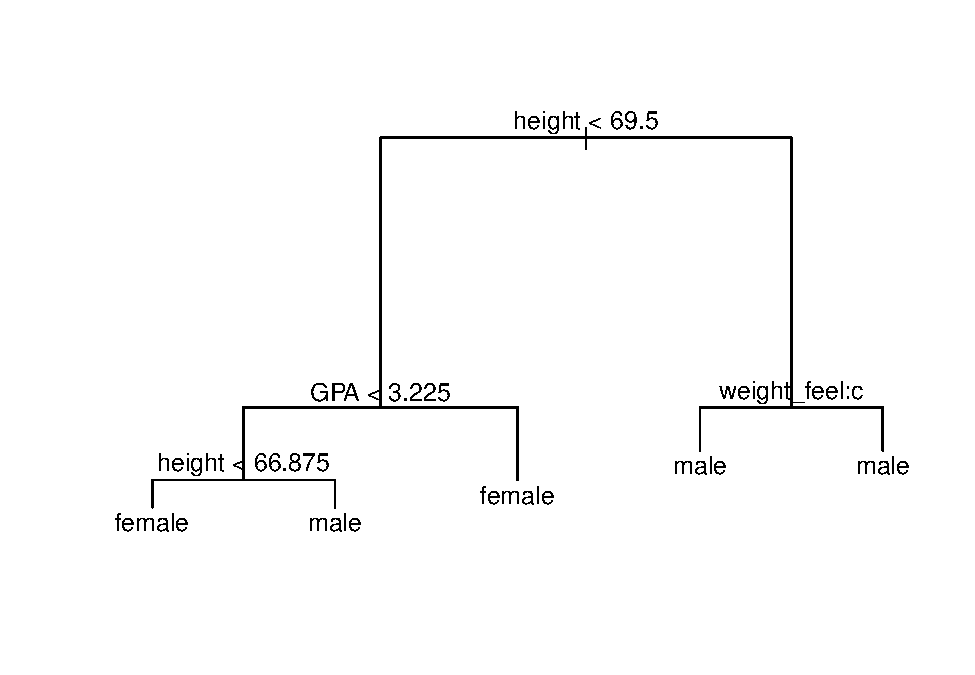
\includegraphics{A_Random_Forest_Model_for_Computer-Assisted_Activity-Recognition_files/figure-latex/unnamed-chunk-5-1} \end{center}
  
  \begin{verbatim}
  3) height > 69.5 28 19.070 male ( 0.1071 0.8929 )  
      6) weight_feel: 3_overweight 10 12.220 male ( 0.3000 0.7000 ) *
      7) weight_feel: 1_underweight,2_about_right 18  0.000 male ( 0.0000 1.0000 ) *
  \end{verbatim}
  
  It may seem odd that the classification tree made a split that ended up
  in two nodes with the same prediction. Why bother making another
  division? The tree still made a split because there was a way to make a
  smaller total deviance. The smaller the deviance of a node leads to
  increased \emph{node purity}. This means that the region could be
  further subdivided into 2 regions where each was more purely male or
  female. After the division, one node is completely male and the other is
  70\% male. If the height is greater than 69.5 inches and they feel
  overweight, then the object being male is absolutely certain. If they
  feel just right or underweight, 70\% of the node are male. Even though
  we are less certain of this classification (compared to 89\% male before
  the division), it improves the deviance. We want the deviance as close
  to 0 as possible and the deviance improved from 19.070 to 12.220. The
  sum of the deviances from the post-division nodes is closer to 0 than
  the pre-division node.
  
  Below is a summary of the classification tree example from above.
  
  \begin{verbatim}
  Classification tree:
  tree(formula = sex ~ fastest + GPA + height + sleep + weight_feel + 
      love_first, data = m111survey)
  Variables actually used in tree construction:
  "height"      "GPA"         "weight_feel"
  Number of terminal nodes:  5 
  Residual mean deviance:  0.4748 = 30.86 / 65 
  Misclassification error rate: 0.1143 = 8 / 70
  \end{verbatim}
  
  The summary given shows the variables actually used in constructing the
  classification tree, the number of terminal nodes, the residual mean
  deviance, and the misclassification error rate.
  
  In order to find the residual mean deviance, R added the deviance at all
  5 terminal nodes and then divided by (number of observations - number of
  terminal nodes). This is a very difficult number to interpret. The main
  thing to understand is that the smaller the residual mean deviance, the
  more ``pure'' the nodes are on average. Thus,
  
  \[ Residual Mean Deviance = \frac{30.869}{70-5} = 0.4749\]
  
  The residual mean deviance (RMD) is also used to compare two different
  tree models and how well they predict. The smaller the value of the
  residual mean deviance, the better the tree is at predicting on its own
  data. For example, if I have one tree model used to predict the sex of
  individual using one dataset and another tree model used to predict if
  an individual is at risk for diabetes using a different dataset, the
  residual mean deviance could be used to compare how well the models will
  predict on its own data. If the RMD of the first model is 0.4749 and the
  RMD of the second model is 0.5812, then we know that the first model is
  better at making predictions.
  
  The final output given by the classification tree summary is the
  misclassification error rate. The performance of a model is measured in
  terms of its misclassification error rate: percentage of incorrectly
  classified instances in the data set (Witten and Eibe, 2000). The lower
  the misclassification error rate, the higher the performance of the
  model. In other words, a lower misclassification rate means that a
  smaller number of objects are being misclassified and the model is
  making correct predictions.
  
  As you can see from the example, classification trees are easy to
  interpret and fairly good predictions can be made from them. In this
  example, the misclassification error rate is about 11.4\%. This means
  that 8 out of 70 observations were misclassified. However, the tree is
  looking at correct answers that were given. If this classification tree
  were given new data, the error rate would most likely be much worse.
  
  Unfortunately, R has some round-off error. This is why the values
  calculated are slightly off from the summary.
  
  \section{The Need for Test Sets}\label{the-need-for-test-sets}
  
  A model should be able to be used to classify new data. Thus, it is
  important to have high model performance with new data. To have a model
  that performs well with new data it is important to divide the original
  data set into two new sets (training and test sets). The \emph{training
  set} is used to build the model and the \emph{test set} is new data that
  is used to measure the model's performance by being treated as new data.
  The model made with the training data will be tried out on the ``new''
  test data. When the original data set is separated into the training and
  test sets, the simplest partition is a two-way random partition, careful
  to avoid introducing any systematic differences. In other words, the
  training set can be created by randomly selecting a portion of the data
  and the test set is created with the remaining points, i.e.~training set
  is made with 20\% of the data and the remaining 80\% makes up the test
  set.
  
  Why not use all the data from the data set? Then more data will be
  available to make the model and the model will be more accurate, right?
  Actually, this is incorrect. The \emph{resubstitution error} (error rate
  on the training set) is a bad predictor of performance on new data
  because the model was built to account for the training data. The best
  model for predicting is the dataset itself. So, if you take a given data
  instance and ask for it's classification, you can look that instance up
  in the dataset and report the correct result every time. You are asking
  the model to make predictions to data that it has ``seen'' before- data
  that were used to create the model. Thus, to really know if the model
  would be a good predictor of the weight lift motion, it must be measured
  on the test data set (the data it has never ``seen'' before), not the
  training set.
  
  Now we're ready to look more at a random forest model and what it does.
  
  \section{Random Forests}\label{random-forests}
  
  \subsection{History and Author}\label{history-and-author}
  
  The algorithm that is used to induce random forests was developed by Leo
  Breiman and Adele Cutler in 2001. Leo Breiman was a distinguished
  statistician at the University of California, Berkeley. Breiman's work
  helped to bridge the gap between statistics and computer science,
  particularly in the field of machine learning. His most important
  contributions were his work on classification trees and ensembles of
  trees through the random forest technique. Adele Cutler is a
  statistician at the University of Utah. Leo Breiman was her PhD advisor
  and they worked together to come up with the random forest technique
  that is most commonly used today (Wikipedia).
  
  Even though Breiman and Cutler created the algorithm for random forests,
  the concept of random forest decision trees was first introduced to the
  mathematical community by Tin Kam Ho of Bell Labs in 1995. The term for
  random forests came from Ho's random decision forests. The development
  of Breiman's algorithm was influenced by Ho's work with random subspace
  selection (Ho, 1995). Brieman was also influenced by the work of Yali
  Amit and Donald Geman, who introduced the idea of searching over a
  random subset of the available decisions when splitting a node, in the
  context of growing a single tree (Amit \& German, 1997). The algorithm
  combines Breiman's ideas and the random selection of features in order
  to construct a collection of decision trees with controlled variance.
  Thus, in Brieman's method a forest of trees is grown, and variation
  among the trees is introduced by projecting the training data into a
  randomly chosen subspace before fitting each tree (Breiman, 2001).
  
  A random forest package was published for R by Andy Liaw and Matthew
  Wiener, based on original Fortran code by Leo Breiman and Adele Cutler.
  The following links to a PDF document for further information on the
  \texttt{randomForest} R package:
  
  \url{https://cran.r-project.org/web/packages/randomForest/randomForest.pdf}
  
  \subsection{How Random Forests Work}\label{how-random-forests-work}
  
  \subsubsection{Tree Splitting}\label{tree-splitting}
  
  Random forests are a way of averaging multiple classification trees,
  which are trained on different parts of the same training set. However,
  there are some major differences in the classification trees used in a
  random forest compared to a regular classification tree. First, at any
  point where the tree is thinking of a split, the tree does not look at
  all the predictor variables. Instead, a random subset of the predictor
  variables is picked. At each node, \(\sqrt{n}\) (where n is the number
  of predictor variables) predictor variables are picked. The floor of
  \(\sqrt{n}\) is the number of predictor variables picked. This means
  that a number is given as the largest integer that is less than or equal
  to \(\sqrt{n}\). While the regular tree examines every predictor
  variable at each node and picks the one that will give the best
  prediction, the random forest tree looks at \(\sqrt{n}\) of predictor
  variables at each node and then picks the one that will give the best
  prediction. Also, this means that most trees in the random forest are
  different. We want the trees to differ from one another. They will make
  errors, but they will be errors in different directions, so to say. The
  hope is that the different trees will ``cancel out'' the error.
  
  As an example, we will look at the weight lifting data. There are over
  100 different predictor variables in this dataset. However, in a later
  section I will do some data cleaning and remove predictor variables that
  are not actually useful. The data cleaning process will leave me with 53
  variables. Thus, in the random forest procedure, whenever a tree is
  thinking about splitting at a node, floor(\(\sqrt{53}\)) predictor
  variables will be used. Since (\(\sqrt{53}\)) is 7.28011, the tree will
  look at 7 of the 53 predictor variables.
  
  \subsubsection{Tree Size}\label{tree-size}
  
  A second important difference between random forest classification trees
  and regular classification trees is the size. Random forest
  classification trees are overgrown. In a regular classification tree the
  \texttt{mincut} is set at 5. In random forests we are looking at trees
  with nodes that end up being very small- one or two objects in the final
  nodes. One example of the arguments in the \texttt{randomForest} package
  is \texttt{nodesize}. This is the minimum size of terminal nodes. The
  default for the classification trees in \texttt{randomForest} is 1.
  
  {[}Note: There is a \texttt{treesize} package that controls tree size in
  regular classification trees. There is also a \texttt{randomForest}
  package argument that controls the tree size in the random forest
  classification trees- \texttt{nodesize}{]}
  
  Thus, larger trees are grown because the terminal nodes can have a
  minimum of 1 object. This overgrowing of classification trees allows for
  great variability in the classification trees. Most of the
  classification trees will not be able to make predictions well on new
  data. In fact, many will have strange results. Even though an individual
  overgrown tree may closely describe the training data, the tree will not
  give good results on new data because it is tracking chance variation as
  pattern. However, putting together all the trees can actually give good
  results. The trees are all tracking chance variation in different
  directions and by putting them together the extreme results can be
  ``cancelled out''.
  
  \subsubsection{Tree Building}\label{tree-building}
  
  A third difference that needs to be considered is the fact that the
  classification trees used to build a random forest do not use the entire
  training data. Rather, they select at random, with replacement, from the
  training data. This random sample size is equal to the size of the
  original training data set. Since each tree does not use the entire
  training data, this gives variability that we want to take into account
  when making a model. The training data set resembles a sample of all the
  possible measurments. So, let's think about the weight lifting data
  which I will use later. The weight lifting data are like a random sample
  of the data we could have gotten while taking measurements of the weight
  lifting subjects. Overall, we want to try to reflect chance variations
  in real-life measurements. However, we don't have all the possible
  observations. We only have the weight lifting data set as an
  approximation. So taking a sample of the data we have is the best
  approximation we have to taking another sample in a real life
  population. Therefore, taking many samples (and most of them end up
  being different from each other) is the best way to see how trees depend
  on chance variation and this variablitity is incorporated into random
  forests. Thus, once again, errors are made but we hope the differences
  in the random samples ``cancel out'' those errors to provide a fairly
  good model for predictions.
  
  The concept of a random sample with the sample size equal to the number
  of observations in a set may seem a little confusing at first. Let me
  illustrate this concept with a simple example:
  
  I will take a random sample, with replacement, from the numbers 1
  through 100. I begin with a list of the first 100 numbers and I put them
  in a bag (this is my original data set). I draw out a number from the
  bag and write it down. I replace the number, pick from the bag again,
  and write down the number I've drawn. I replace the number and continue
  in this way until I have a new list of 100 numbers (this is the sample
  data set). The new list may have duplicate numbers or some numbers may
  be missing entirely. This new list is an example of what it would be
  like to take a random sample from those 100 numbers.
  
  I have made a list of 100 numbers and taken a random sample from the
  original list.
  
  \begin{verbatim}
  "27" "11" "97" "36" "64" "4"  "9"  "6"  "71"  "25" 
  "52" "82" "3"  "62" "66" "45" "2"  "3"  "99"  "14" 
  "66" "23" "37" "34" "92" "46" "96" "69" "61"  "84" 
  "17" "44" "36" "86" "9"  "58" "52" "59" "84"  "45" 
  "19" "66" "60" "37" "37" "61" "11" "81" "100" "46" 
  "10" "49" "60" "79" "21" "62" "21" "89" "22"  "54" 
  "2"  "75" "33" "56" "67" "14" "9"  "58" "31"  "25" 
  "89" "95" "39" "51" "45" "96" "23" "36" "87"  "35" 
  "72" "8"  "46" "94" "31" "97" "7"  "30" "46"  "32" 
  "46" "56" "16" "28" "16" "80" "72" "40" "47"  "4"  
  \end{verbatim}
  
  Notice that some of the numbers have been repeated and some numbers are
  missing. We can have the computer look at the numbers we are missing and
  the numbers that are included in the random sample.
  
  \newpage
  
  Below is a table showing the numbers that are missing from the random
  sample:
  
  \begin{verbatim}
   "1"  "5"  "12" "13" "15" "18"
   "20" "24" "26" "29" "38" "41"
   "42" "43" "48" "50" "53" "55"
   "57" "63" "65" "68" "70" "73"
   "74" "76" "77" "78" "83" "85"
   "88" "90" "91" "93" "98" 
  \end{verbatim}
  
  Below is a table showing the numbers that are part of the random sample:
  
  \begin{verbatim}
  
   "27" "11" "97" "36"  "64" "4"  "9"  "6"  "71" "25"  "52" 
   "82" "3"  "62" "66"  "45" "2"  "99" "14" "23" "37"  "34" 
   "92" "46" "96" "69"  "61" "84" "17" "44" "86" "58"  "59" 
   "19" "60" "81" "100" "10" "49" "79" "21" "89" "22"  "54" 
   "75" "33" "56" "67"  "31" "95" "39" "51" "87" "35"  "72" 
   "8"  "94" "7"  "30"  "32" "16" "28" "80" "40" "47"  
  \end{verbatim}
  
  Notice that 35 numbers are missing from the new list, which is 35\% of
  the data.
  
  Why don't we take another sample of 100?
  
  I have made another list of 100 numbers and taken a random sample from
  the original list.
  
  \begin{verbatim}
  "90" "27" "38" "58" "91" "21" "90" "95" "67"  "63" 
  "7"  "21" "18" "69" "39" "77" "50" "72" "100" "39" 
  "78" "94" "22" "66" "13" "27" "39" "2"  "39"  "87" 
  "35" "49" "60" "50" "19" "83" "67" "80" "11"  "73" 
  "42" "83" "65" "79" "56" "53" "79" "3"  "48"  "74" 
  "70" "48" "87" "44" "25" "8"  "10" "32" "52"  "67" 
  "41" "92" "30" "46" "34" "66" "26" "48" "77"  "9"  
  "88" "34" "84" "35" "34" "48" "90" "87" "39"  "78" 
  "97" "44" "72" "40" "33" "76" "21" "72" "13"  "25" 
  "15" "24" "6"  "65" "88" "78" "80" "46" "42"  "82"
  \end{verbatim}
  
  Below is a table showing the numbers that are missing from the random
  sample:
  
  \begin{verbatim}
  
   "1"  "4"  "5"  "12" "14" "16"
   "17" "20" "23" "28" "29" "31"
   "36" "37" "43" "45" "47" "51"
   "54" "55" "57" "59" "61" "62"
   "64" "68" "71" "75" "81" "85"
   "86" "89" "93" "96" "98" "99"
  \end{verbatim}
  
  Below is a table showing the numbers that are part of the random sample:
  
  \begin{verbatim}
  "90"  "27" "38" "58" "91" "21" "95" "67"
  "63"  "7"  "18" "69" "39" "77" "50" "72"
  "100" "78" "94" "22" "66" "13" "2"  "87"
  "35"  "49" "60" "19" "83" "80" "11" "73"
  "42"  "65" "79" "56" "53" "3"  "48" "74"
  "70"  "44" "25" "8"  "10" "32" "52" "41"
  "92"  "30" "46" "34" "26" "9"  "88" "84"
  "97"  "40" "33" "76" "15" "24" "6"  "82"   
  \end{verbatim}
  
  Notice that this list is missing 36 numbers from the original list. This
  means 36\% of the original data is missing. In fact, the expected
  proportion of missing data is about 0.3678 or better known as
  \(\frac{1}{e}\). The number \emph{e} is an important mathematical
  constant that is the base of the natural logarithm. It is approximately
  equal to 2.71828. {[}Note: The history and mathematical importance of
  the number \emph{e} is not in the scope of this paper, but if you would
  like to know more I suggest reading ``e: the Story of a Number'' by Eli
  Maor (1994).{]}
  
  Now let's see what happens when we take a larger sample. Suppose I have
  a list of numbers 1 to 10,000 instead of only 100. Then, looking at the
  numbers included in the new list, we find that 3,681 are missing.
  
  As you can see in the table below, after performing 10 random samples
  with replacement of size 10,000 the amount of missing numbers stays
  around 3600 (or about 36\%). These are also close to the proportion of
  \(\frac{1}{e}\). In fact, as the size of a dataset increases, the closer
  the proportion of missing data gets to \(\frac{1}{e}\).
  
  \begin{verbatim}
   "3682" "3674" "3690" "3691" "3727"
   "3696" "3596" "3685" "3716" "3741"
  \end{verbatim}
  
  Below is the computation done by R to show the value of \(\frac{1}{e}\):
  
  \begin{verbatim}
  0.3678794
  \end{verbatim}
  
  As an added bonus, the random sample with replacement is used to make an
  estimation of how well the random forest will do. And that estimation
  will be made even when the random forest is being constructed.
  
  Thus, the random selection of predictor variables, the overgrowing of
  the trees and the random sample of data allows for many different
  possibilities, which can help with making predictions. This makes the
  random forest a very effective modeling tool.
  
  \subsection{Summary of How Random Forests
  Work}\label{summary-of-how-random-forests-work}
  
  This summarizes the information from above.
  
  \begin{enumerate}
  \def\labelenumi{\arabic{enumi}.}
  \item
    Each tree is trained on roughly \(2/3^{\text{rd}}\) of the total
    training data. Cases are drawn at random with replacement from the
    original training data. This sample will be the training set for
    growing the tree. The other \(1/3^{\text{rd}}\) of the cases are left
    out of the sample (recall it will actually be about \(\frac{1}{e}\) of
    the data). For each tree, using the leftover data, the
    misclassification rate (or out-of-bag error rate) is calculated. The
    error from all trees is used to determine overall OOB error rate for
    the classification.This out-of-bag (OOB) data is used to get a running
    unbiased estimate of the classification error as trees are added to
    the forest. It is also used to get estimates of variable importance.
  \item
    Some predictor variables (say, m) are selected at random out of all
    the predictor variables and the best split on these m is used to split
    the node. By default, m is square root of the total number of all
    predictors for classification. The value of m is held constant during
    the forest growing. As explained earlier, in a standard classification
    tree, each split is created after examining every variable and picking
    the best split from all the variables.
  \item
    Each tree gives a classification, and we say the tree ``votes'' for
    that class. The forest chooses the classification having the most
    votes over all the trees in the forest. The vote will be YES or NO.
    All the YES votes are counted and this is the predicted probability
    for a classification.
  \item
    The classification trees that make up the random forest are overgrown
    to allow for greater variability in the classification trees. While
    the individual overgrown trees make poor predictions on data, putting
    together hundreds of overgrown trees can ``cancel out'' the extreme
    results and better predictions can be made.
  \end{enumerate}
  
  \subsection{An Extended Random Forest
  Example}\label{an-extended-random-forest-example}
  
  Once again we will use all the data from the \texttt{m111survey} to
  construct a random forest. However, for the weight lifting data I will
  make a division for training and test sets before constructing a random
  forest.
  
  Below is an example of the code for random forests, along with
  explanations for each part.
  
  The code for implementing a random forest:
  
  \begin{Shaded}
  \begin{Highlighting}[]
  \KeywordTok{set.seed}\NormalTok{(}\DecValTok{1010}\NormalTok{)}
    \CommentTok{# set.seed() keeps the results of the code chunk the same. This}
    \CommentTok{# is useful when reproducible results are desired.}
  
  \NormalTok{rf.sexm111 <-}\StringTok{ }\KeywordTok{randomForest}\NormalTok{(sex~fastest+GPA+height+sleep+}
  \StringTok{                             }\NormalTok{weight_feel+}
  \StringTok{                             }\NormalTok{love_first+extra_life+ideal_ht+}
  \StringTok{                             }\NormalTok{seat+enough_Sleep+diff.ideal.act., }
                               \DataTypeTok{data=}\NormalTok{m111surv2, }\DataTypeTok{ntree=}\DecValTok{500}\NormalTok{)}
  \end{Highlighting}
  \end{Shaded}
  
  The \texttt{randomForest} function has several arguments, but only some
  are used in this example. The first argument, \texttt{formula}, is a
  formula describing the model to be fitted. We want to predict sex of an
  individual based on the variables of fastest speed ever driven, GPA,
  height, the amount of sleep the participant got the night before, how
  the participant feels about their weight, if the participant believes in
  love at first sight, if the participant believes in extraterrestrial
  life, the participant's ideal height, where the participant prefers to
  sit in class, if the participant believes they got enough sleep the
  night before and the difference between ideal height and actual height.
  The structure for the formula is as follows:
  
  \begin{verbatim}
  sex~fastest+GPA+height+sleep+
       weight_feel+
       love_first+extra_life+ideal_ht+
       seat+enough_Sleep+diff.ideal.act
       
  \end{verbatim}
  
  The next argument is \texttt{data}. This is the data frame containing
  the variables in the model. As stated earlier, the data frame for this
  example is taken from the MAT 111 Survey data.
  
  The final argument used in this example is \texttt{ntree}, which is the
  number of trees to grow. The default number of trees to be grown for the
  random forest is 500, but this can be adjusted.
  
  The random forest is put into an object,\texttt{rf.sexm111}, thay way we
  don't have to write out all the components every time we want to
  implement the random forest. Also, \texttt{set.seed} is used to
  reproduce the results of the random forest output. In other words, each
  time the code is executed the results will be the same.
  
  \newpage
  
  Now that the code has been written out, we can take a look at the
  results. Below is the output given by running the random forest code:
  
  \begin{verbatim}
  randomForest(formula = sex ~ fastest + GPA + height + sleep +      
  weight_feel + love_first + extra_life + ideal_ht + seat +      
  enough_Sleep + diff.ideal.act., data = m111surv2, ntree = 500) 
                 
  Type of random forest: classification
  
  Number of trees: 500
  
  No. of variables tried at each split: 3
  
  
  OOB estimate of  error rate: 4.41%
  
  Confusion matrix:
         female male class.error
  female     37    1  0.02631579
  male        2   28  0.06666667
  \end{verbatim}
  
  Let's talk about what happened bit by bit. Recall that the
  \texttt{randomForest} function is stored in an object
  (\texttt{rf.sexm111}) and R prints out the object as output with several
  different components.
  
  First, is the \texttt{call} which is the original call to
  \texttt{randomForest}, or the code to implement the function.
  
  \begin{verbatim}
  
  randomForest(formula = sex ~ fastest + GPA + height + sleep +      
  weight_feel + love_first + extra_life + ideal_ht + seat +      
  enough_Sleep + diff.ideal.act., data = m111surv2, ntree = 500) 
  \end{verbatim}
  
  Second, the \texttt{type} is given. This refers to the types of trees
  that were grown for the random forest. Trees are usually grown as
  classification or regression trees. However, it is not necessary to
  understand the difference between the two for our purposes. In this
  example, the trees are classification trees.
  
  \begin{verbatim}
  Type of random forest: classification
  \end{verbatim}
  
  Third, the number of tres grown, \texttt{ntree} is given. The default
  number is 500. However, depending on the model this number can be
  changed.
  
  \begin{verbatim}
  Number of trees: 500
  \end{verbatim}
  
  We can actually look at some of the individual trees constructed for the
  random forest and see some of the differences between them:
  
  \newpage
  
  \begin{longtable}[c]{@{}rrlrrl@{}}
  \caption{Tree 1 made by the Random Forest}\tabularnewline
  \toprule
  LD & RD & split var & split point & status & prediction\tabularnewline
  \midrule
  \endfirsthead
  \toprule
  LD & RD & split var & split point & status & prediction\tabularnewline
  \midrule
  \endhead
  2 & 3 & GPA & 3.715 & 1 & NA\tabularnewline
  4 & 5 & ideal\_ht & 71.000 & 1 & NA\tabularnewline
  0 & 0 & NA & 0.000 & -1 & female\tabularnewline
  6 & 7 & height & 66.875 & 1 & NA\tabularnewline
  8 & 9 & height & 77.000 & 1 & NA\tabularnewline
  0 & 0 & NA & 0.000 & -1 & female\tabularnewline
  10 & 11 & weight\_feel & 1.000 & 1 & NA\tabularnewline
  0 & 0 & NA & 0.000 & -1 & male\tabularnewline
  12 & 13 & weight\_feel & 2.000 & 1 & NA\tabularnewline
  0 & 0 & NA & 0.000 & -1 & male\tabularnewline
  14 & 15 & seat & 1.000 & 1 & NA\tabularnewline
  0 & 0 & NA & 0.000 & -1 & male\tabularnewline
  0 & 0 & NA & 0.000 & -1 & female\tabularnewline
  0 & 0 & NA & 0.000 & -1 & male\tabularnewline
  0 & 0 & NA & 0.000 & -1 & female\tabularnewline
  \bottomrule
  \end{longtable}
  
  The \emph{left daughter (LD)} and the \emph{right daughter (RD)} are the
  two nodes that are made by a division. The \emph{split var} is the
  variable for which the division was made. The \emph{split point} is the
  point where the split was made. The \emph{status} shows if more
  divisions will be made (1) or if a node is terminal (-1). And then the
  final column shows the prediction of a terminal node. This is true for
  the two other tables shown below.
  
  \begin{longtable}[c]{@{}rrlrrl@{}}
  \caption{Tree 250 made by the Random Forest}\tabularnewline
  \toprule
  LD & RD & split var & split point & status & prediction\tabularnewline
  \midrule
  \endfirsthead
  \toprule
  LD & RD & split var & split point & status & prediction\tabularnewline
  \midrule
  \endhead
  2 & 3 & height & 66.875 & 1 & NA\tabularnewline
  4 & 5 & ideal\_ht & 72.500 & 1 & NA\tabularnewline
  6 & 7 & diff.ideal.act. & 1.750 & 1 & NA\tabularnewline
  0 & 0 & NA & 0.000 & -1 & female\tabularnewline
  0 & 0 & NA & 0.000 & -1 & male\tabularnewline
  8 & 9 & weight\_feel & 1.000 & 1 & NA\tabularnewline
  0 & 0 & NA & 0.000 & -1 & male\tabularnewline
  0 & 0 & NA & 0.000 & -1 & male\tabularnewline
  10 & 11 & height & 72.500 & 1 & NA\tabularnewline
  0 & 0 & NA & 0.000 & -1 & female\tabularnewline
  0 & 0 & NA & 0.000 & -1 & male\tabularnewline
  \bottomrule
  \end{longtable}
  
  \newpage
  
  \begin{longtable}[c]{@{}rrlrrl@{}}
  \caption{Tree 500 made by the Random Forest}\tabularnewline
  \toprule
  LD & RD & split var & split point & status & prediction\tabularnewline
  \midrule
  \endfirsthead
  \toprule
  LD & RD & split var & split point & status & prediction\tabularnewline
  \midrule
  \endhead
  2 & 3 & extra\_life & 1.00 & 1 & NA\tabularnewline
  4 & 5 & ideal\_ht & 69.00 & 1 & NA\tabularnewline
  6 & 7 & ideal\_ht & 70.00 & 1 & NA\tabularnewline
  0 & 0 & NA & 0.00 & -1 & female\tabularnewline
  0 & 0 & NA & 0.00 & -1 & male\tabularnewline
  8 & 9 & sleep & 4.75 & 1 & NA\tabularnewline
  0 & 0 & NA & 0.00 & -1 & male\tabularnewline
  0 & 0 & NA & 0.00 & -1 & female\tabularnewline
  0 & 0 & NA & 0.00 & -1 & female\tabularnewline
  \bottomrule
  \end{longtable}
  
  Notice that each tree is different. The variables used for division
  differ for each tree. One tree may use variables that make the
  prediction off in one way, but another tree may use variables that make
  the prediction off in another way. Since 500 trees are used to make up
  this random forest, the mistakes even out to make a fairly good
  prediction model.
  
  The fourth component of the output is \texttt{mtry}. This is the number
  of predictors sampled for splitting at each node. The default value for
  this argument is \(\sqrt{n}\).
  
  \begin{verbatim}
  
  No. of variables tried at each split: 3
  \end{verbatim}
  
  Recall that whenever a tree is thinking about splitting at a node,
  floor(\(\sqrt{n}\)) predictor variables will be used. Since
  \(\sqrt{11}\) = 3.3166, 3 variables are tried at each possible split.
  
  Fifth, an error rate is given. Recall that the misclassification rate is
  calculated using the leftover data using the leftover data from the
  random sample with replacement and the error from all trees is used to
  determine overall OOB error rate for the classification.
  
  \begin{verbatim}
  
  OOB estimate of  error rate: 4.41%
  \end{verbatim}
  
  The final output of this example is the confusion matrix of the
  out-of-bag error. This tells us how many times the prediction of sex was
  correct or incorrect and gives an error rate for each classification.
  
  \begin{verbatim}
  Confusion matrix:
  
         female male class.error
  
  female     37    1  0.02631579
  
  male        2   28  0.06666667
  \end{verbatim}
  
  This table shows us that for all the females in the data set, the random
  forest classified 37 correctly as female and only misclassified one
  female as male. Also, only two males were misclassified as females.
  
  \emph{This RF was constructed using only a training set. We only have
  the OOB error rate as an estimate of how it would do on new data.
  However, with the weight lifting data I will make a division into
  training and test sets.}
  
  \section{Computing Tools}\label{computing-tools}
  
  For this project I use a variety of tools which include R, RStudio, Git,
  and GitHub.
  
  \subsection{Expansion on R-related
  Tools}\label{expansion-on-r-related-tools}
  
  R is a programming language and an open source statisical program
  software environment used for statistical computing. R provides a wide
  variety of statistical and graphical techniques. R is available as Free
  Software under the terms of the Free Software Foundation's GNU General
  Public License. It compiles and runs on a variety of systems, such as
  UNIX, Windows, and MacOS.
  
  To learn more about R and its contributors, please visit:
  \url{https://www.r-project.org/}.
  
  R Studio is a free and open source integrated development environment
  (IDE) for R. This is a programmer's tool to help make writing and
  formatting code an easier task.
  
  To learn more about RStudio, please visit:
  \url{https://www.rstudio.com/}.
  
  I am using R Markdown, which is an authoring format that enables easy
  creation of dynamic documents, presentations, and reports from R. This
  document format is extremely useful for a statistical paper (which is
  what I will be working on this year), as it allows me to enter code
  chunks that are automatically executed as well as add figures, graphs,
  and charts. This format also allows me to save PDF, HTML, and Word
  versions of my document. However, this format is not very flexible when
  it comes to the aesthetics of the document. I cannot easily format my
  Bibliography nor do I know how to indent paragraphs because I am just
  beginning to use RMarkdown. If you require certain format for this
  paper, please understand that it will be very difficult with RMarkdown
  and I will probably not be able to focus on that until much later.
  
  To learn more about R Markdown, please visit:
  \url{http://rmarkdown.rstudio.com/}.
  
  \subsection{Expansion on Git and
  GitHub}\label{expansion-on-git-and-github}
  
  Git is a free and open source distributed version control system
  designed to handle everything from small to very large projects with
  speed and efficiency.
  
  To learn more about Git, please visit: \url{https://git-scm.com/}.
  
  GitHub is a web-based Git repository hosting service. It offers all of
  the distributed revision control and source code management (SCM)
  functionality of Git. Unlike Git, which is strictly a command-line tool,
  GitHub provides a web-based graphical interface and desktop. It also
  provides access control and several collaboration features such as bug
  tracking, feature requests, task management, and wikis for every
  project. GitHub offers both plans for private repositories and free
  accounts, which are usually used to host open-source software projects.
  
  To learn more about GitHub, please visit: \url{https://github.com/}.
  
  \chapter{Results}\label{results}
  
  The following sections will go through the implementation of the methods
  described from earlier.
  
  \section{Data Cleaning}\label{data-cleaning}
  
  Many of the following steps for downloading and cleaning the data are
  taken from the report ``Predicting Movement-Types: Quick Model-Making
  with Random Forests'' written by Dr.~White.
  
  \subsection{Downloading}\label{downloading}
  
  The main data, along with the examination data, can be downloaded from
  the web:
  
  \begin{quote}
  \url{http://groupware.les.inf.puc-rio.br/har}
  \end{quote}
  
  Below is an example of the code used to download, read, and load a data
  file into R.
  
  \begin{Shaded}
  \begin{Highlighting}[]
  \NormalTok{weblink <-}\StringTok{ }\KeywordTok{paste0}\NormalTok{(}\StringTok{"http://groupware.les.inf.puc-rio.br/static/WLE/"}\NormalTok{,}
                    \StringTok{"WearableComputing_weight_lifting_exercises_biceps"}\NormalTok{,}
                     \StringTok{"_curl_variations.csv"}\NormalTok{)}
  \NormalTok{wl <-}\StringTok{ }\KeywordTok{read.csv}\NormalTok{(weblink, }\DataTypeTok{stringsAsFactors =} \OtherTok{FALSE}\NormalTok{)}
  \KeywordTok{save}\NormalTok{(wl, }\DataTypeTok{file =} \StringTok{"data/CopyOfwl.rda"}\NormalTok{)}
  \end{Highlighting}
  \end{Shaded}
  
  \subsection{Elimination of Variables}\label{elimination-of-variables}
  
  The main data set consists of 19622 observations on 160 variables,
  including:
  
  \begin{itemize}
  \tightlist
  \item
    a row-number variable \texttt{X};
  \item
    \texttt{user\_name} (the name of the subject);
  \item
    three time-stamp variables;
  \item
    two variables, \texttt{new\_window} and \texttt{num\_window} related
    to time-windows;
  \item
    152 numerical measurements derived from the inertial measurement units
    (IMUs);
  \item
    the variable \texttt{classe} that records the activity-type.
  \end{itemize}
  
  Many of the variables can be removed because they are not actually
  useful as predictor variables. For this data set, the row-number
  variable \texttt{X}, the time-stamp variables, and the
  \texttt{new\_window} variable are not particularly useful for predicting
  the lift motion. Also, for many of the variables the values are
  altogether missing. These variables appear to be summaries of other
  variables, such as kurtosis, averages, maximums, minimums, skewness
  values, amplitude values, variances, and standard deviations. Although
  these summaries may have predictive value, it is difficult to see how to
  take advantage of this fact, so we will simply exclude all such
  variables from our training data.
  
  \emph{Note: Kurtosis is a measure of the ``tailedness'' of the
  probability distribution of a real-valued random variable}
  (\url{http://mathworld.wolfram.com/Kurtosis.html})
  
  \newpage
  
  The spurious variables can be eliminated from our data frame. The code
  for this is as follows:
  
  \begin{Shaded}
  \begin{Highlighting}[]
  \CommentTok{# This function determines which of the variables have values}
  \CommentTok{# that are mostly assigned.}
  
  \NormalTok{goodVar <-}\StringTok{ }\NormalTok{function(x)\{}
    \NormalTok{mostly_assigned <-}\StringTok{ }\KeywordTok{sum}\NormalTok{(}\KeywordTok{is.na}\NormalTok{(x))/}\KeywordTok{length}\NormalTok{(x) <}\StringTok{ }\FloatTok{0.5}
    \NormalTok{mostly_nonblank <-}\StringTok{ }\KeywordTok{sum}\NormalTok{(x ==}\StringTok{ ""}\NormalTok{)/}\KeywordTok{length}\NormalTok{(x) <}\StringTok{ }\FloatTok{0.5}
    \KeywordTok{return}\NormalTok{(mostly_assigned &&}\StringTok{ }\NormalTok{mostly_nonblank)}
  \NormalTok{\}                   }
  
  \NormalTok{not_summary_variable <-}\StringTok{ }\KeywordTok{sapply}\NormalTok{(wl, }\DataTypeTok{FUN =} \NormalTok{goodVar) }
    \CommentTok{# This identifies all the variables }
    \CommentTok{# that do not have missing values.}
  
  \NormalTok{goodNames <-}\StringTok{ }\KeywordTok{names}\NormalTok{(not_summary_variable[not_summary_variable])}
  
  \NormalTok{keepNames <-}\StringTok{ }\NormalTok{goodNames[-}\KeywordTok{c}\NormalTok{(}\DecValTok{1}\NormalTok{,}\DecValTok{3}\NormalTok{,}\DecValTok{4}\NormalTok{,}\DecValTok{5}\NormalTok{,}\DecValTok{6}\NormalTok{)] }
    \CommentTok{# This keeps all the useful variables in }
    \CommentTok{# the data set and removes the extra variables that are }
    \CommentTok{# not useful.}
  
  \NormalTok{wl2 <-}\StringTok{ }\NormalTok{wl[,keepNames]}
    \CommentTok{# All the variables we wish to keep will be put into a new}
    \CommentTok{# data set so as to preserve the original data set.}
  
  \NormalTok{wl2$user_name <-}\StringTok{ }\KeywordTok{factor}\NormalTok{(wl$user_name) }
  \NormalTok{wl2$classe <-}\StringTok{ }\KeywordTok{factor}\NormalTok{(wl$classe)}
    \CommentTok{# Makes user_name and classe a factor variable }
    \CommentTok{# because the randomForest function requires factors.}
  
  \NormalTok{wn <-}\StringTok{ }\NormalTok{wl$num_window }
    \CommentTok{# I will want to separate my data into training and test sets }
    \CommentTok{# based on the num_window variable.}
  \end{Highlighting}
  \end{Shaded}
  
  \newpage
  
  \section{Data Separation}\label{data-separation}
  
  The data set I am working with will have to be divided into two sets (a
  training set and a test set). The training set is used to build the
  model and the test set is data that is used to measure the model's
  performance by being treated as ``new'' data. The model made with the
  training data will be tried out on the ``new'' test data. When the
  original data set is separated into the training and test sets, the
  simplest partition is a two-way random partition, careful to avoid
  introducing any systematic differences. The reasoning behind this type
  of division is that the data available for analytics fairly represents
  the real-world processes and that those processes are expected to remain
  stable over time (Steinberg, 2014). So, a well-constructed model will
  perform adequately on the new data.
  
  Why not use all the data from the data set? Then more data will be
  available to make the model and the model will be more accurate, right?
  However, if you recall from section 2.3, The Need for Test Sets, this is
  incorrect. The \emph{resubstitution error} (error rate on the training
  set) is a bad predictor of performance on new data because the model was
  built to account for the training data. The best model for predicting is
  the dataset itself. So, if you take a given instance and ask for it's
  classification, you can look that instance up in the dataset and report
  the correct result every time. In essence, you are asking the model to
  make predictions to data that it has ``seen'' before- data that were
  used to create the model. Thus, to really know if the model would be a
  good predictor of the weight lift motion, it must be measured on the
  test data set, not the training set.
  
  Since there are six subjects in the study, a total of 300 lifts were
  performed and recorded (each subject did 10 repetitions of the 5 lifts).
  However, during \textbf{each} lift the IMU measurements were gathered
  using a sliding window approach with different lengths (from 0.5 to 2.5
  seconds), with a 0.5 second overlap. This resulted in a large data set
  (over 19,000 observations); a single observation in the data set
  corresponds to a specific time window for a specific subject performing
  one of the specified lifts. While the simplest division is to separate
  the original data set into training and test sets using a random
  partition (a typical separation), an expanded separation will be done to
  make the model more ``honest''.
  
  I decided to separate my data by window number. In real life we test on
  a new lift. So, when we divide into test and training sets, we ideally
  want to keep individual lifts separate- no portion of a lift in the test
  and training set. Even though there is no way for us to tell when a new
  lift is beginning, we have the window number which provides long
  portions of a lift and allows for a separation with little cross-over.
  
  \newpage
  
  Below is a function that has been written for easy separation. The
  arguments of this function are the data set to be separated and the
  variable by which the separation will be done. I can then use this
  function to separate the weight lifting data set into training and test
  sets by the \texttt{num\_window} variable.
  
  \begin{Shaded}
  \begin{Highlighting}[]
  \CommentTok{# Function for separation by variable.}
  
  \NormalTok{partition_var <-}\StringTok{ }\NormalTok{function(data, var)\{}
    \NormalTok{vals <-}\StringTok{ }\KeywordTok{unique}\NormalTok{(var) }
      \CommentTok{# Returns a vector that is the same as "var", but with}
      \CommentTok{# duplicate elements removed.}
    
    \NormalTok{n <-}\StringTok{ }\KeywordTok{length}\NormalTok{(vals)  }
      \CommentTok{# Gives the size of the "vals" vector.}
    
    \NormalTok{m <-}\StringTok{ }\KeywordTok{floor}\NormalTok{(}\DecValTok{2}\NormalTok{/}\DecValTok{3}\NormalTok{*n) }
      \CommentTok{# This will be used to help separate the data; 2/3 in a training }
      \CommentTok{# set and 1/3 in a test set.}
    
    \NormalTok{bools <-}\StringTok{ }\KeywordTok{c}\NormalTok{(}\KeywordTok{rep}\NormalTok{(}\OtherTok{TRUE}\NormalTok{,m), }\KeywordTok{rep}\NormalTok{(}\OtherTok{FALSE}\NormalTok{,n-m))  }
      \CommentTok{# A booliean object that has m TRUE}
      \CommentTok{# values and n-m FALSE values. Thus it is the same size as "vals".}
      \CommentTok{# This will be used later to help determine which rows of the }
      \CommentTok{# "var" data will be included in each set of separation.}
      \CommentTok{# Since there are m TRUEs, 2/3 of the "vals" will be used in the}
      \CommentTok{# training set and 1/3 will be used in the test set.}
    
    \NormalTok{inTrain <-}\StringTok{ }\KeywordTok{sample}\NormalTok{(bools, }\DataTypeTok{size =} \NormalTok{n, }\DataTypeTok{replace =} \OtherTok{FALSE}\NormalTok{) }
      \CommentTok{# Since it is not good enough to just}
      \CommentTok{# take the first 2/3 of the "bools" vector and put it into a }
      \CommentTok{# training set a random sample of the "bools" with size n }
      \CommentTok{# and no replacement is taken. This includes the same }
      \CommentTok{# information as "bools", but it has been all mixed up. }
    
    \NormalTok{trvals <-}\StringTok{ }\NormalTok{vals[inTrain] }
      \CommentTok{# Gives values to the list of TRUEs from the inTrain }
      \CommentTok{# random sample. "trvals" includes the "vals" that had been }
      \CommentTok{# labeled TRUE in the "inTrain" vector.}
    
    \NormalTok{vartr <-}\StringTok{ }\NormalTok{var %in%}\StringTok{ }\NormalTok{trvals }
      \CommentTok{# A vector of TRUEs and FALSEs. This will label which of the }
      \CommentTok{# "var" values were TRUE in "trvals". }
    
    \NormalTok{tr <-}\StringTok{ }\NormalTok{data[vartr,] }
      \CommentTok{# Training data set- a data frame that includes rows of "vartr".}
    
    \NormalTok{tst <-}\StringTok{ }\NormalTok{data[!vartr,] }
      \CommentTok{# Test data set- a data frame that includes rows that are not}
      \CommentTok{# in "vartr".}
    
    \KeywordTok{return}\NormalTok{(}\KeywordTok{list}\NormalTok{(tr, tst)) }
      \CommentTok{# Since an R function can only return one object, a list of }
      \CommentTok{# the training and test sets is returned.}
  \NormalTok{\}}
  \end{Highlighting}
  \end{Shaded}
  
  \newpage 
  
  Now the data can be separated into the training and test sets and used
  for a random forest procedure:
  
  \begin{Shaded}
  \begin{Highlighting}[]
  \KeywordTok{set.seed}\NormalTok{(}\DecValTok{2020}\NormalTok{)}
    \CommentTok{# set.seed() keeps the results of the code chunk the same. This}
    \CommentTok{# is useful when reproducible results are desired.}
  
  \NormalTok{results <-}\StringTok{ }\KeywordTok{partition_var}\NormalTok{(wl2, wn) }
    \CommentTok{# I put the num_window variable into a new object, wn }
  
  \NormalTok{wlTrain <-}\StringTok{ }\NormalTok{results[[}\DecValTok{1}\NormalTok{]] }
    \CommentTok{# Since 2 results are given (test and training set), }
    \CommentTok{# the first result is the training set}
  
  \NormalTok{wlTest <-}\StringTok{ }\NormalTok{results[[}\DecValTok{2}\NormalTok{]]  }
    \CommentTok{# The second result is the test set}
  
  \NormalTok{rf <-}\StringTok{ }\KeywordTok{randomForest}\NormalTok{(}\DataTypeTok{x =} \NormalTok{wlTrain[,}\DecValTok{1}\NormalTok{:}\DecValTok{53}\NormalTok{], }\DataTypeTok{y =} \NormalTok{wlTrain$classe, }
                     \DataTypeTok{xtest =} \NormalTok{wlTest[,}\DecValTok{1}\NormalTok{:}\DecValTok{53}\NormalTok{], }\DataTypeTok{ytest =} \NormalTok{wlTest$classe)}
  \end{Highlighting}
  \end{Shaded}
  
  \begin{verbatim}
  Call:
   randomForest(x = wlTrain[, 1:53], y = wlTrain$classe,
                xtest = wlTest[, 1:53], ytest = wlTest$classe) 
  \end{verbatim}
  
  This formula includes the training and the test sets that we created
  earlier.
  
  \begin{verbatim}
  Type of random forest: classification
  
  Number of trees: 500
  
  No. of variables tried at each split: 7
  \end{verbatim}
  
  Unsuprisingly, we used 500 classification trees to make up the random
  forest. Also, since 53 variables are used in the data set, 7 variables
  were tried at each possible split of the classification trees. \newpage
  
  Now, the error rates and confusion matrices are shown below:
  
  \begin{longtable}[c]{@{}lrrrrrr@{}}
  \caption{Confusion matrix for Training Set}\tabularnewline
  \toprule
  & A & B & C & D & E & class.error\tabularnewline
  \midrule
  \endfirsthead
  \toprule
  & A & B & C & D & E & class.error\tabularnewline
  \midrule
  \endhead
  A & 3683 & 1 & 0 & 0 & 0 & 0.0002714\tabularnewline
  B & 1 & 2348 & 1 & 0 & 0 & 0.0008511\tabularnewline
  C & 0 & 3 & 2123 & 0 & 0 & 0.0014111\tabularnewline
  D & 0 & 0 & 5 & 2280 & 0 & 0.0021882\tabularnewline
  E & 0 & 0 & 0 & 2 & 2553 & 0.0007828\tabularnewline
  \bottomrule
  \end{longtable}
  
  \begin{verbatim}
  OOB estimate of  error rate: 0.1%
  \end{verbatim}
  
  \begin{longtable}[c]{@{}lrrrrrr@{}}
  \caption{Confusion matrix for Test Set}\tabularnewline
  \toprule
  & A & B & C & D & E & class.error\tabularnewline
  \midrule
  \endfirsthead
  \toprule
  & A & B & C & D & E & class.error\tabularnewline
  \midrule
  \endhead
  A & 1857 & 38 & 1 & 0 & 0 & 0.0205696\tabularnewline
  B & 29 & 1379 & 39 & 0 & 0 & 0.0469938\tabularnewline
  C & 3 & 134 & 1143 & 13 & 3 & 0.1180556\tabularnewline
  D & 0 & 0 & 31 & 889 & 11 & 0.0451128\tabularnewline
  E & 0 & 8 & 0 & 16 & 1028 & 0.0228137\tabularnewline
  \bottomrule
  \end{longtable}
  
  \begin{verbatim}
  Test set error rate: 4.92%
  \end{verbatim}
  
  For your reference, here is a list of the lift types:
  
  \begin{verbatim}
  * Class A: correct lift movement
  * Class B: throwing the elbows to the front
  * Class C: lifting the dumbbell only halfway
  * Class D: lowering the dumbbell only halfway
  * Class E: throwing the hips to the front
  \end{verbatim}
  
  Notice that very few misclassification errors are made on the training
  set---13 errors out of thousands of classifications. However, when
  looking at the confusion matrix for the test set, many more errors are
  made. For example, in the first confusion matrix, the model only made 3
  errors when classifying a lift as a Class C error (misclassified it as a
  Class B error). The overall class error rate for C is about 0.1\%. But
  in the second confusion matrix (test set) 3 Class C errors were
  misclassified as a correct lift, 134 were misclassified as a Class B
  error, 13 as a Class D error, and 3 as a Class E error. Overall, the
  class error rate for C is about 11\%. The classification rate is not as
  good for the test set as it is for the training set.
  
  However, this is not surprising. The classification trees for the random
  forest were grown using the data from the training set. They predicted
  on the same window numbers that they were trained on. Therefore, they
  had already ``seen'' the window numbers and the trees made few errors
  because of it. When the trees began predicting on the test data the
  misclassifications increase. Recall, the resubstitution error (error
  rate on the training set) is a bad predictor of performance on new data
  because the model was built to account for the training data. So, even
  though the error rate is worse when using the test set, it is in fact a
  better estimate on how this model would work on new lifts by the
  experiment subjects.
  
  \chapter*{Conclusion and Further
  Discussion}\label{conclusion-and-further-discussion}
  \addcontentsline{toc}{chapter}{Conclusion and Further Discussion}
  
  Recall that Dr.~White devised a random forest model to predict
  activity-type from the same variables used in my random forest model.
  The final model he constructed was estimated to be correct about 99.7\%
  of the time. Dr.~White built the model using observations from the same
  lifts as the observations for which the activity-type was predicted, and
  he recognized that this was not an optimal model for predicting lift
  type for the subjects should they return to the gym and perform new
  lifts. That is where my research project began; I wanted to build an
  ``honest'' predictive model to use in realistic circumstances.
  
  The main goal of this project was to find a model that could test
  accurately on new lifts. In essence, this goal was met. In real life, a
  model would have to be able to predict the lift classification using
  data gathered from new lifts by the subjects. Even though there is no
  way to tell when a new lift is beginning, the window number provides
  long portions of a lift and allows for a separation with little
  cross-over. This gives a good representation of what it would be like to
  test on new lifts. The model was less accurate because we are testing on
  different parts of the lift than before. If a way to separate the data
  by complete window numbers, then I would suspect that the model would do
  even worse. But, it would be an even more realistic estimation. Thus, it
  was found separating by even part of a lift has an impact on the
  predictive model.
  
  \section{Further Discussion}\label{further-discussion}
  
  The model in this project is a more ``realistic'' model than Dr.~White's
  original model, but it is used for classifying new lift types from the
  same subjects. It is not a very good model for predicting the lift types
  of new subjects. We can get a feel for how the model would predict on
  new subjects by creating a model where 5 of the test subjects are used
  as training data and 1 subject is used as test data. This would give 6
  different random forest models (since there are 6 subjects). However,
  this model would most likely give horrible results.
  
  \subsection{A Look at How This Model Would Work on New
  Subjects}\label{a-look-at-how-this-model-would-work-on-new-subjects}
  
  The plan to implement this idea is as follows:
  
  \begin{itemize}
  \tightlist
  \item
    Use all of the data (training and test combined).
  \item
    Divide it into six folds. Each fold will contains all of the
    observations pertaining to a particular subject.
  \item
    For each subject, build a 500-tree random forest on the other five
    subjects, then test it on the fold for the subject.
  \item
    We will NOT use user\_name to build our forests.
  \item
    We'll get six sets of error-rates. These will give us some idea of how
    a model built on our six subjects might do for a new subject.
  \end{itemize}
  
  Here is the first random forest. The data from the subject Adelmo will
  be the test set.
  
  \begin{Shaded}
  \begin{Highlighting}[]
  \KeywordTok{set.seed}\NormalTok{(}\DecValTok{3030}\NormalTok{)}
  \NormalTok{subjects <-}\StringTok{ }\KeywordTok{levels}\NormalTok{(wl2$user_name)}
  
  \NormalTok{Sub1 <-}\StringTok{ }\NormalTok{wl2[wl2$user_name ==}\StringTok{ }\NormalTok{subjects[}\DecValTok{1}\NormalTok{], ]}
  \NormalTok{OtherSubs1 <-}\StringTok{ }\NormalTok{wl2[wl2$user_name !=}\StringTok{ }\NormalTok{subjects[}\DecValTok{1}\NormalTok{], ]}
  \NormalTok{forest1 <-}\StringTok{ }\KeywordTok{randomForest}\NormalTok{(}\DataTypeTok{x =} \NormalTok{OtherSubs1[, }\DecValTok{2}\NormalTok{:}\DecValTok{53}\NormalTok{], }\DataTypeTok{y =} \NormalTok{OtherSubs1$classe,}
                                 \DataTypeTok{xtest =} \NormalTok{Sub1[, }\DecValTok{2}\NormalTok{:}\DecValTok{53}\NormalTok{], }
                                 \DataTypeTok{ytest =} \NormalTok{Sub1$classe,}
                                 \DataTypeTok{ntree =} \DecValTok{500}\NormalTok{)}
  \end{Highlighting}
  \end{Shaded}
  
  \newpage
  
  \begin{verbatim}
  Call:
    randomForest(x = OtherSubs1[, 2:53], y = OtherSubs1$classe, 
        xtest = Sub1[, 2:53], ytest = Sub1$classe, ntree = 500) 
                 
  Type of random forest: classification
  
  Number of trees: 500
  
  No. of variables tried at each split: 7
  \end{verbatim}
  
  \begin{longtable}[c]{@{}lrrrrrr@{}}
  \caption{Confusion matrix for Training Set-Adelmo}\tabularnewline
  \toprule
  & A & B & C & D & E & class.error\tabularnewline
  \midrule
  \endfirsthead
  \toprule
  & A & B & C & D & E & class.error\tabularnewline
  \midrule
  \endhead
  A & 4414 & 0 & 0 & 0 & 1 & 0.0002265\tabularnewline
  B & 4 & 3017 & 0 & 0 & 0 & 0.0013241\tabularnewline
  C & 0 & 3 & 2669 & 0 & 0 & 0.0011228\tabularnewline
  D & 0 & 0 & 9 & 2691 & 1 & 0.0037023\tabularnewline
  E & 0 & 0 & 0 & 4 & 2917 & 0.0013694\tabularnewline
  \bottomrule
  \end{longtable}
  
  \begin{verbatim}
  OOB estimate of  error rate: 0.14%
  \end{verbatim}
  
  \begin{longtable}[c]{@{}lrrrrrr@{}}
  \caption{Confusion matrix for Test Set-Adelmo}\tabularnewline
  \toprule
  & A & B & C & D & E & class.error\tabularnewline
  \midrule
  \endfirsthead
  \toprule
  & A & B & C & D & E & class.error\tabularnewline
  \midrule
  \endhead
  A & 0 & 0 & 0 & 0 & 1165 & 1.0000000\tabularnewline
  B & 2 & 32 & 0 & 0 & 742 & 0.9587629\tabularnewline
  C & 0 & 0 & 0 & 0 & 750 & 1.0000000\tabularnewline
  D & 0 & 0 & 0 & 0 & 515 & 1.0000000\tabularnewline
  E & 0 & 0 & 0 & 0 & 686 & 0.0000000\tabularnewline
  \bottomrule
  \end{longtable}
  
  \begin{verbatim}
  Test set error rate: 81.55%
  \end{verbatim}
  
  Since the call for the random forest is similar for all subjects and the
  type of trees used, the number of trees used, and the number of
  variables tried at each split are the same, only the confusion matrices
  will be shown for the rest of the random forests.
  
  The next random forest uses the data from Carlitos as the test set.
  
  \begin{Shaded}
  \begin{Highlighting}[]
  \KeywordTok{set.seed}\NormalTok{(}\DecValTok{3131}\NormalTok{)}
  
  \NormalTok{Sub2 <-}\StringTok{ }\NormalTok{wl2[wl2$user_name ==}\StringTok{ }\NormalTok{subjects[}\DecValTok{2}\NormalTok{], ]}
  \NormalTok{OtherSubs2 <-}\StringTok{ }\NormalTok{wl2[wl2$user_name !=}\StringTok{ }\NormalTok{subjects[}\DecValTok{2}\NormalTok{], ]}
  \NormalTok{forest2 <-}\StringTok{ }\KeywordTok{randomForest}\NormalTok{(}\DataTypeTok{x =} \NormalTok{OtherSubs2[, }\DecValTok{2}\NormalTok{:}\DecValTok{53}\NormalTok{], }\DataTypeTok{y =} \NormalTok{OtherSubs2$classe,}
                                 \DataTypeTok{xtest =} \NormalTok{Sub2[, }\DecValTok{2}\NormalTok{:}\DecValTok{53}\NormalTok{], }
                                 \DataTypeTok{ytest =} \NormalTok{Sub2$classe,}
                                 \DataTypeTok{ntree =} \DecValTok{500}\NormalTok{)}
  \end{Highlighting}
  \end{Shaded}
  
  \begin{longtable}[c]{@{}lrrrrrr@{}}
  \caption{Confusion matrix for Training Set-Carlitos}\tabularnewline
  \toprule
  & A & B & C & D & E & class.error\tabularnewline
  \midrule
  \endfirsthead
  \toprule
  & A & B & C & D & E & class.error\tabularnewline
  \midrule
  \endhead
  A & 4746 & 0 & 0 & 0 & 0 & 0.0000000\tabularnewline
  B & 2 & 3105 & 0 & 0 & 0 & 0.0006437\tabularnewline
  C & 0 & 4 & 2925 & 0 & 0 & 0.0013657\tabularnewline
  D & 0 & 0 & 9 & 2720 & 1 & 0.0036630\tabularnewline
  E & 0 & 0 & 0 & 3 & 2995 & 0.0010007\tabularnewline
  \bottomrule
  \end{longtable}
  
  \begin{verbatim}
  OOB estimate of  error rate: 0.12%
  \end{verbatim}
  
  \begin{longtable}[c]{@{}lrrrrrr@{}}
  \caption{Confusion matrix for Test Set-Carlitos}\tabularnewline
  \toprule
  & A & B & C & D & E & class.error\tabularnewline
  \midrule
  \endfirsthead
  \toprule
  & A & B & C & D & E & class.error\tabularnewline
  \midrule
  \endhead
  A & 828 & 6 & 0 & 0 & 0 & 0.0071942\tabularnewline
  B & 239 & 383 & 8 & 1 & 59 & 0.4449275\tabularnewline
  C & 290 & 76 & 122 & 3 & 2 & 0.7525355\tabularnewline
  D & 417 & 19 & 4 & 40 & 6 & 0.9176955\tabularnewline
  E & 232 & 168 & 1 & 33 & 175 & 0.7126437\tabularnewline
  \bottomrule
  \end{longtable}
  
  \begin{verbatim}
  Test set error rate: 50.26%
  \end{verbatim}
  
  The next random forest uses the data from Charles as the test set.
  
  \begin{Shaded}
  \begin{Highlighting}[]
  \KeywordTok{set.seed}\NormalTok{(}\DecValTok{3232}\NormalTok{)}
  
  \NormalTok{Sub3 <-}\StringTok{ }\NormalTok{wl2[wl2$user_name ==}\StringTok{ }\NormalTok{subjects[}\DecValTok{3}\NormalTok{], ]}
  \NormalTok{OtherSubs3 <-}\StringTok{ }\NormalTok{wl2[wl2$user_name !=}\StringTok{ }\NormalTok{subjects[}\DecValTok{3}\NormalTok{], ]}
  \NormalTok{forest3 <-}\StringTok{ }\KeywordTok{randomForest}\NormalTok{(}\DataTypeTok{x =} \NormalTok{OtherSubs3[, }\DecValTok{2}\NormalTok{:}\DecValTok{53}\NormalTok{], }\DataTypeTok{y =} \NormalTok{OtherSubs3$classe,}
                                 \DataTypeTok{xtest =} \NormalTok{Sub3[, }\DecValTok{2}\NormalTok{:}\DecValTok{53}\NormalTok{], }
                                 \DataTypeTok{ytest =} \NormalTok{Sub3$classe,}
                                 \DataTypeTok{ntree =} \DecValTok{500}\NormalTok{)}
  \end{Highlighting}
  \end{Shaded}
  
  \begin{longtable}[c]{@{}lrrrrrr@{}}
  \caption{Confusion matrix for Training Set-Charles}\tabularnewline
  \toprule
  & A & B & C & D & E & class.error\tabularnewline
  \midrule
  \endfirsthead
  \toprule
  & A & B & C & D & E & class.error\tabularnewline
  \midrule
  \endhead
  A & 4680 & 0 & 0 & 0 & 1 & 0.0002136\tabularnewline
  B & 2 & 3048 & 2 & 0 & 0 & 0.0013106\tabularnewline
  C & 0 & 4 & 2879 & 0 & 0 & 0.0013874\tabularnewline
  D & 0 & 0 & 6 & 2568 & 0 & 0.0023310\tabularnewline
  E & 0 & 0 & 0 & 2 & 2894 & 0.0006906\tabularnewline
  \bottomrule
  \end{longtable}
  
  \begin{verbatim}
  OOB estimate of  error rate: 0.11%
  \end{verbatim}
  
  \newpage
  
  \begin{longtable}[c]{@{}lrrrrrr@{}}
  \caption{Confusion matrix for Test Set-Charles}\tabularnewline
  \toprule
  & A & B & C & D & E & class.error\tabularnewline
  \midrule
  \endfirsthead
  \toprule
  & A & B & C & D & E & class.error\tabularnewline
  \midrule
  \endhead
  A & 821 & 7 & 0 & 71 & 0 & 0.0867631\tabularnewline
  B & 208 & 463 & 0 & 74 & 0 & 0.3785235\tabularnewline
  C & 275 & 120 & 0 & 141 & 3 & 1.0000000\tabularnewline
  D & 461 & 149 & 0 & 29 & 3 & 0.9548287\tabularnewline
  E & 88 & 0 & 0 & 0 & 623 & 0.1237693\tabularnewline
  \bottomrule
  \end{longtable}
  
  \begin{verbatim}
  Test set error rate: 45.25%
  \end{verbatim}
  
  The next random forest uses the data from Eurico as the test set.
  
  \begin{Shaded}
  \begin{Highlighting}[]
  \KeywordTok{set.seed}\NormalTok{(}\DecValTok{3333}\NormalTok{)}
  
  \NormalTok{Sub4 <-}\StringTok{ }\NormalTok{wl2[wl2$user_name ==}\StringTok{ }\NormalTok{subjects[}\DecValTok{4}\NormalTok{], ]}
  \NormalTok{OtherSubs4 <-}\StringTok{ }\NormalTok{wl2[wl2$user_name !=}\StringTok{ }\NormalTok{subjects[}\DecValTok{4}\NormalTok{], ]}
  \NormalTok{forest4 <-}\StringTok{ }\KeywordTok{randomForest}\NormalTok{(}\DataTypeTok{x =} \NormalTok{OtherSubs4[, }\DecValTok{2}\NormalTok{:}\DecValTok{53}\NormalTok{], }\DataTypeTok{y =} \NormalTok{OtherSubs4$classe,}
                                 \DataTypeTok{xtest =} \NormalTok{Sub4[, }\DecValTok{2}\NormalTok{:}\DecValTok{53}\NormalTok{], }
                                 \DataTypeTok{ytest =} \NormalTok{Sub4$classe,}
                                 \DataTypeTok{ntree =} \DecValTok{500}\NormalTok{)}
  \end{Highlighting}
  \end{Shaded}
  
  \begin{longtable}[c]{@{}lrrrrrr@{}}
  \caption{Confusion matrix for Training Set-Eurico}\tabularnewline
  \toprule
  & A & B & C & D & E & class.error\tabularnewline
  \midrule
  \endfirsthead
  \toprule
  & A & B & C & D & E & class.error\tabularnewline
  \midrule
  \endhead
  A & 4715 & 0 & 0 & 0 & 0 & 0.0000000\tabularnewline
  B & 3 & 3200 & 2 & 0 & 0 & 0.0015601\tabularnewline
  C & 0 & 5 & 2928 & 0 & 0 & 0.0017047\tabularnewline
  D & 0 & 0 & 11 & 2622 & 1 & 0.0045558\tabularnewline
  E & 0 & 0 & 0 & 4 & 3061 & 0.0013051\tabularnewline
  \bottomrule
  \end{longtable}
  
  \begin{verbatim}
  OOB estimate of  error rate: 0.16%
  \end{verbatim}
  
  \begin{longtable}[c]{@{}lrrrrrr@{}}
  \caption{Confusion matrix for Test Set-Eurico}\tabularnewline
  \toprule
  & A & B & C & D & E & class.error\tabularnewline
  \midrule
  \endfirsthead
  \toprule
  & A & B & C & D & E & class.error\tabularnewline
  \midrule
  \endhead
  A & 121 & 13 & 0 & 0 & 731 & 0.8601156\tabularnewline
  B & 0 & 0 & 0 & 0 & 592 & 1.0000000\tabularnewline
  C & 0 & 0 & 0 & 0 & 489 & 1.0000000\tabularnewline
  D & 11 & 0 & 0 & 0 & 571 & 1.0000000\tabularnewline
  E & 2 & 7 & 0 & 0 & 533 & 0.0166052\tabularnewline
  \bottomrule
  \end{longtable}
  
  \begin{verbatim}
  Test set error rate: 78.7%
  \end{verbatim}
  
  \newpage
  
  The next random forest uses the data from Jeremy as the test set.
  
  \begin{Shaded}
  \begin{Highlighting}[]
  \KeywordTok{set.seed}\NormalTok{(}\DecValTok{3434}\NormalTok{)}
  
  \NormalTok{Sub5 <-}\StringTok{ }\NormalTok{wl2[wl2$user_name ==}\StringTok{ }\NormalTok{subjects[}\DecValTok{5}\NormalTok{], ]}
  \NormalTok{OtherSubs5 <-}\StringTok{ }\NormalTok{wl2[wl2$user_name !=}\StringTok{ }\NormalTok{subjects[}\DecValTok{5}\NormalTok{], ]}
  \NormalTok{forest5 <-}\StringTok{ }\KeywordTok{randomForest}\NormalTok{(}\DataTypeTok{x =} \NormalTok{OtherSubs5[, }\DecValTok{2}\NormalTok{:}\DecValTok{53}\NormalTok{], }\DataTypeTok{y =} \NormalTok{OtherSubs5$classe,}
                                 \DataTypeTok{xtest =} \NormalTok{Sub5[, }\DecValTok{2}\NormalTok{:}\DecValTok{53}\NormalTok{], }
                                 \DataTypeTok{ytest =} \NormalTok{Sub5$classe,}
                                 \DataTypeTok{ntree =} \DecValTok{500}\NormalTok{)}
  \end{Highlighting}
  \end{Shaded}
  
  \begin{longtable}[c]{@{}lrrrrrr@{}}
  \caption{Confusion matrix for Training Set-Jeremy}\tabularnewline
  \toprule
  & A & B & C & D & E & class.error\tabularnewline
  \midrule
  \endfirsthead
  \toprule
  & A & B & C & D & E & class.error\tabularnewline
  \midrule
  \endhead
  A & 4402 & 0 & 0 & 0 & 1 & 0.0002271\tabularnewline
  B & 4 & 3304 & 0 & 0 & 0 & 0.0012092\tabularnewline
  C & 0 & 5 & 2764 & 1 & 0 & 0.0021661\tabularnewline
  D & 0 & 0 & 9 & 2684 & 1 & 0.0037120\tabularnewline
  E & 0 & 0 & 0 & 1 & 3044 & 0.0003284\tabularnewline
  \bottomrule
  \end{longtable}
  
  \begin{verbatim}
  OOB estimate of  error rate: 0.14%
  \end{verbatim}
  
  \begin{longtable}[c]{@{}lrrrrrr@{}}
  \caption{Confusion matrix for Test Set-Jeremy}\tabularnewline
  \toprule
  & A & B & C & D & E & class.error\tabularnewline
  \midrule
  \endfirsthead
  \toprule
  & A & B & C & D & E & class.error\tabularnewline
  \midrule
  \endhead
  A & 765 & 409 & 0 & 3 & 0 & 0.3500425\tabularnewline
  B & 17 & 446 & 21 & 0 & 5 & 0.0879346\tabularnewline
  C & 0 & 392 & 242 & 18 & 0 & 0.6288344\tabularnewline
  D & 0 & 426 & 34 & 60 & 2 & 0.8850575\tabularnewline
  E & 0 & 284 & 26 & 187 & 65 & 0.8843416\tabularnewline
  \bottomrule
  \end{longtable}
  
  \begin{verbatim}
  Test set error rate: 53.62%
  \end{verbatim}
  
  The final random forest uses the data from Pedro as the test set.
  
  \begin{Shaded}
  \begin{Highlighting}[]
  \KeywordTok{set.seed}\NormalTok{(}\DecValTok{3535}\NormalTok{)}
  
  \NormalTok{Sub6 <-}\StringTok{ }\NormalTok{wl2[wl2$user_name ==}\StringTok{ }\NormalTok{subjects[}\DecValTok{6}\NormalTok{], ]}
  \NormalTok{OtherSubs6 <-}\StringTok{ }\NormalTok{wl2[wl2$user_name !=}\StringTok{ }\NormalTok{subjects[}\DecValTok{6}\NormalTok{], ]}
  \NormalTok{forest6 <-}\StringTok{ }\KeywordTok{randomForest}\NormalTok{(}\DataTypeTok{x =} \NormalTok{OtherSubs6[, }\DecValTok{2}\NormalTok{:}\DecValTok{53}\NormalTok{], }\DataTypeTok{y =} \NormalTok{OtherSubs6$classe,}
                                 \DataTypeTok{xtest =} \NormalTok{Sub6[, }\DecValTok{2}\NormalTok{:}\DecValTok{53}\NormalTok{],}
                                 \DataTypeTok{ytest =} \NormalTok{Sub6$classe,}
                                 \DataTypeTok{ntree =} \DecValTok{500}\NormalTok{)}
  \end{Highlighting}
  \end{Shaded}
  
  \newpage
  
  \begin{longtable}[c]{@{}lrrrrrr@{}}
  \caption{Confusion matrix for Training Set-Pedro}\tabularnewline
  \toprule
  & A & B & C & D & E & class.error\tabularnewline
  \midrule
  \endfirsthead
  \toprule
  & A & B & C & D & E & class.error\tabularnewline
  \midrule
  \endhead
  A & 4939 & 0 & 0 & 0 & 1 & 0.0002024\tabularnewline
  B & 3 & 3286 & 3 & 0 & 0 & 0.0018226\tabularnewline
  C & 0 & 7 & 2916 & 0 & 0 & 0.0023948\tabularnewline
  D & 0 & 0 & 5 & 2741 & 1 & 0.0021842\tabularnewline
  E & 0 & 0 & 0 & 2 & 3108 & 0.0006431\tabularnewline
  \bottomrule
  \end{longtable}
  
  \begin{verbatim}
  OOB estimate of  error rate: 0.13%
  \end{verbatim}
  
  \begin{longtable}[c]{@{}lrrrrrr@{}}
  \caption{Confusion matrix for Test Set-Pedro}\tabularnewline
  \toprule
  & A & B & C & D & E & class.error\tabularnewline
  \midrule
  \endfirsthead
  \toprule
  & A & B & C & D & E & class.error\tabularnewline
  \midrule
  \endhead
  A & 13 & 53 & 0 & 0 & 574 & 0.9796875\tabularnewline
  B & 31 & 32 & 0 & 0 & 442 & 0.9366337\tabularnewline
  C & 0 & 99 & 0 & 0 & 400 & 1.0000000\tabularnewline
  D & 0 & 81 & 0 & 8 & 380 & 0.9829424\tabularnewline
  E & 0 & 13 & 0 & 2 & 482 & 0.0301811\tabularnewline
  \bottomrule
  \end{longtable}
  
  \begin{verbatim}
  Test set error rate: 79.5%
  \end{verbatim}
  
  Notice that the error rates for all of the forests are quite terrible
  when they predict on a new subject. This model probably would not be
  good to use on new subjects.
  
  \subsection{A Look at Principal Component
  Analysis}\label{a-look-at-principal-component-analysis}
  
  Principal component analysis (PCA) is a useful tool for describing data.
  \emph{Principal component analysis} refers to the statistical procedure
  that uses an orthogonal (perpendicular) transformation to convert a set
  of observations of possibly correlated variables into a set of values of
  linearly uncorrelated variables called principal \textbf{components}.
  This transformation is defined in such a way that the first principal
  component has the largest possible variance (that is, accounts for as
  much of the variability in the data as possible), and each succeeding
  component in turn has the highest variance possible under the constraint
  that it is orthogonal to the preceding components (James, et. al, 2013).
  In other words, PCA transforms the data into a new, lower-dimensional
  subspace--into a new coordinate system. In the new coordinate system,
  the first axis corresponds to the first principal component, which is
  the component that explains the greatest amount of the variance in the
  data. The number of principal components is less than or equal to the
  number of original variables.
  
  A simple example may be helpful in demonstrating what PCA accomplishes
  (Hamilton, 2014).
  
  Suppose we have a data set with only two variables (Figure 2).
  
  \begin{figure}[htbp]
  \centering
  \includegraphics{http://www.lauradhamilton.com/posts/2014/pca-original-dataset.png}
  \caption{Dataset with two variables, x1 and x2}
  \end{figure}
  
  Now, we want to identify the first principal component that explains the
  highest amount of variance. Graphically, if a line is drawn that splits
  the oval lengthwise, that line signifies the component that explains the
  most variance:
  
  \begin{figure}[htbp]
  \centering
  \includegraphics{http://www.lauradhamilton.com/posts/2014/pca-first-principal-component.png}
  \caption{Finding the first principal component}
  \end{figure}
  
  \newpage
  
  To find the second principal component, we find a second line that
  explain the next highest amount of variance. This must be orthogonal to
  the first principal component. The second principal component attempts
  to capture the variance that is not captured by the first principal
  component.
  
  \begin{figure}[htbp]
  \centering
  \includegraphics{http://www.lauradhamilton.com/posts/2014/pca-second-principal-component.png}
  \caption{Finding the second principal component}
  \end{figure}
  
  As you can see in Figure 4, the two principal components are orthogonal
  and capture the elements of the data set.
  
  \newpage
  
  Thus, if PCA was performed on this dataset and the original dataset was
  projected onto the first two principal components, then no information
  would be lost. (A two-dimensional dataset is being transformed to a new
  two-dimensional dataset.) Since there are only two variables in the
  dataset, there can only be two principal components. Figure 5 shows what
  the original dataset projected onto the principal components looks like.
  
  \begin{figure}[htbp]
  \centering
  \includegraphics{http://www.lauradhamilton.com/posts/2014/pca-projected-to-two-dimensions.png}
  \caption{Original dataset projected onto the principal components}
  \end{figure}
  
  \newpage
  
  For the weight lifting data set, we will look at the principal
  components (using commands from the \texttt{FactoMineR} package).
  
  \begin{Shaded}
  \begin{Highlighting}[]
  \NormalTok{wl.pca <-}\StringTok{ }\KeywordTok{PCA}\NormalTok{(wl2[, -}\KeywordTok{c}\NormalTok{(}\DecValTok{1}\NormalTok{,}\DecValTok{2}\NormalTok{,}\DecValTok{55}\NormalTok{)], }\DataTypeTok{graph =} \OtherTok{FALSE}\NormalTok{)}
  
  \CommentTok{# This command runs PCA on the training set. Three variables have}
  \CommentTok{# been removed- `user_name`, `num_window`, and `classe`. The }
  \CommentTok{# predictors must be numerical in order to perform PCA, which is why  }
  \CommentTok{# `user_name` and `classe` were removed. The window numbers were }
  \CommentTok{# removed because they do not contribute to any variance, they are }
  \CommentTok{# just markers for new lifts.}
  \end{Highlighting}
  \end{Shaded}
  
  \begin{longtable}[c]{@{}lrr@{}}
  \caption{The first ten principal components and the percentage of
  variance that each contributes.}\tabularnewline
  \toprule
  & percentage of variance & cumulative percentage of
  variance\tabularnewline
  \midrule
  \endfirsthead
  \toprule
  & percentage of variance & cumulative percentage of
  variance\tabularnewline
  \midrule
  \endhead
  comp 1 & 16.070155 & 16.07015\tabularnewline
  comp 2 & 15.583292 & 31.65345\tabularnewline
  comp 3 & 8.992345 & 40.64579\tabularnewline
  comp 4 & 7.941611 & 48.58740\tabularnewline
  comp 5 & 7.022997 & 55.61040\tabularnewline
  comp 6 & 5.776076 & 61.38648\tabularnewline
  comp 7 & 4.307617 & 65.69409\tabularnewline
  comp 8 & 3.986191 & 69.68028\tabularnewline
  comp 9 & 3.302367 & 72.98265\tabularnewline
  comp 10 & 2.901580 & 75.88423\tabularnewline
  \bottomrule
  \end{longtable}
  
  Apparently, the first five components contribute to a little more than
  half of the variance in our numerical predictors. The first ten
  principal components contribute about 76\% of the variance.
  
  Figure 6 shows some of the most important variables plotted against the
  first two principal components. As seen in the factor map,
  \texttt{yaw\_belt}, \texttt{roll\_belt}, \texttt{total\_accel\_belt},
  \texttt{accel\_belt\_y}, and \texttt{accel\_belt\_z} would be the best
  at spreading out the data. It would be interesting to see what a
  physicist has to say about the variables and if it makes sense that
  these variables are most important for predicting the classifications of
  lift types.
  
  \newpage
  
  \begin{Shaded}
  \begin{Highlighting}[]
  \KeywordTok{plot}\NormalTok{(wl.pca, }\DataTypeTok{choix =} \StringTok{"var"}\NormalTok{, }\DataTypeTok{select =} \StringTok{"cos2 5"}\NormalTok{)}
  \end{Highlighting}
  \end{Shaded}
  
  \begin{figure}
  
  {\centering 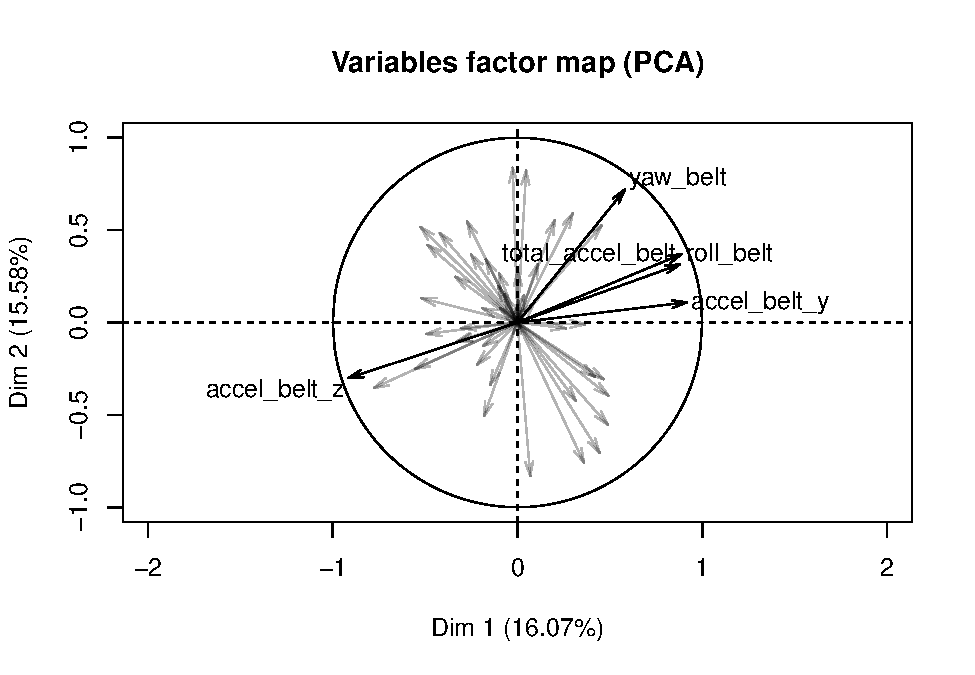
\includegraphics{A_Random_Forest_Model_for_Computer-Assisted_Activity-Recognition_files/figure-latex/unnamed-chunk-51-1} 
  
  }
  
  \caption[The plotting dimensions are determined by the first two principal compnents]{The plotting dimensions are determined by the first two principal compnents.  The labeled variables are the five that are 'closest' to the plane of the these components.}\label{fig:unnamed-chunk-51}
  \end{figure}
  
  \begin{Shaded}
  \begin{Highlighting}[]
  \CommentTok{# Draws the Multiple Correspondence Analysis (MCA) graphs.}
  \CommentTok{# wl.pc is the object we want to use for the plot. "var" tells the }
  \CommentTok{# function to graph the variables. The select argument can be used in }
  \CommentTok{# order to select a part of the elements (individuals if you draw the }
  \CommentTok{# graph of individuals, or variables if you draw the graph of }
  \CommentTok{# variables) that are drawn. select = "cos2 5" and then the 5 }
  \CommentTok{# elements that have the highest cos2 on the 2 dimensions of your }
  \CommentTok{# plot are drawn.}
  \end{Highlighting}
  \end{Shaded}
  
  \newpage
  
  We can also look at the first three principal components and get a
  3-dimensional cloud for each subject. (One outlier was removed in order
  to give a better depiction of the clouds.)
  
  \begin{Shaded}
  \begin{Highlighting}[]
  \KeywordTok{cloud}\NormalTok{(Comp}\FloatTok{.1} \NormalTok{~}\StringTok{ }\NormalTok{Comp}\FloatTok{.2} \NormalTok{*}\StringTok{ }\NormalTok{Comp}\FloatTok{.3}\NormalTok{, }\DataTypeTok{groups =} \NormalTok{wl2$user_name,}
        \DataTypeTok{screen =} \KeywordTok{list}\NormalTok{(}\DataTypeTok{x =} \DecValTok{0}\NormalTok{, }\DataTypeTok{y =} \DecValTok{0}\NormalTok{, }\DataTypeTok{z =} \DecValTok{0}\NormalTok{),}
        \DataTypeTok{auto.key =} \KeywordTok{list}\NormalTok{(}\DataTypeTok{space =} \StringTok{"right"}\NormalTok{),}
        \DataTypeTok{main =} \StringTok{"PC-Plot of Training Data,}\CharTok{\textbackslash{}n}\StringTok{by Subject"}\NormalTok{)}
  \end{Highlighting}
  \end{Shaded}
  
  \begin{figure}
  
  {\centering 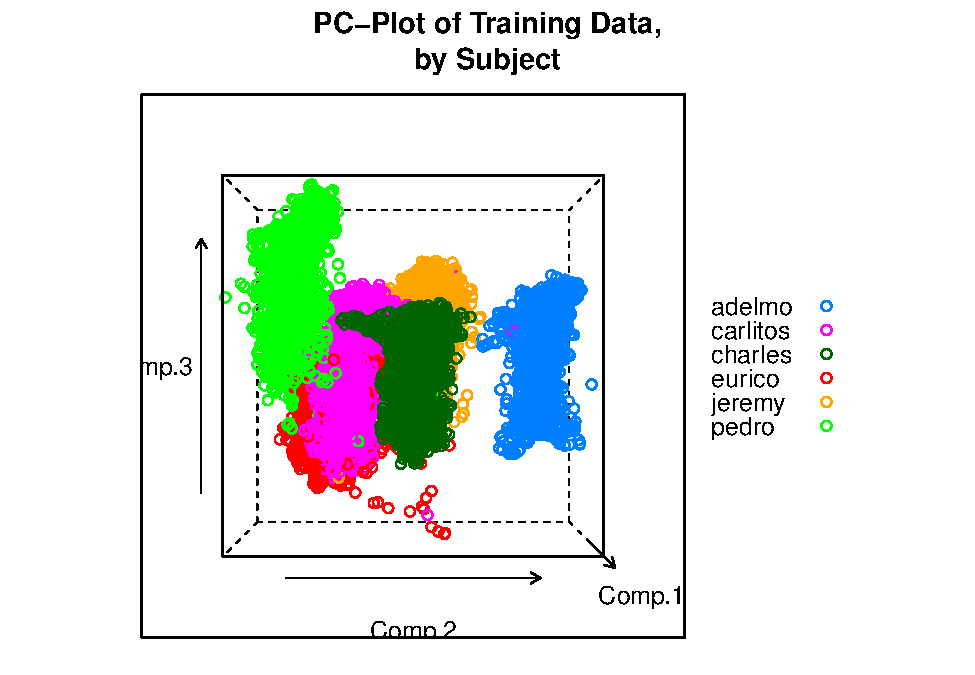
\includegraphics{A_Random_Forest_Model_for_Computer-Assisted_Activity-Recognition_files/figure-latex/unnamed-chunk-53-1} 
  
  }
  
  \caption[View of the training observations, plotted in the first three principal components]{View of the training observations, plotted in the first three principal components.  Observations are colored according to which subject was being observed.  Obviously the six subjects have rather distinct movement profiles.}\label{fig:unnamed-chunk-53}
  \end{figure}
  
  Each subject has distinct movement profiles, so it would be difficult to
  predict the movements of one subject from the movements of the other
  subjects. It is interesting to note that Adelmo and Pedro had two of the
  worst error rates from the random forest procedure and their clouds are
  removed from the others.
  
  \appendix
  
  \chapter{Hidden Code Chunks}\label{hidden-code-chunks}
  
  This appendix includes all of the R chunks of code that were hidden
  throughout the document (using the \texttt{include\ =\ FALSE} chunk tag)
  to help with readibility and/or setup.
  
  \begin{Shaded}
  \begin{Highlighting}[]
  \CommentTok{# These are the required packages.}
  
  \KeywordTok{library}\NormalTok{(FactoMineR)}
  \KeywordTok{library}\NormalTok{(randomForest)}
  \KeywordTok{library}\NormalTok{(caret)}
  \KeywordTok{library}\NormalTok{(knitr)}
  \KeywordTok{library}\NormalTok{(tree)}
  \KeywordTok{library}\NormalTok{(tigerstats)}
  \end{Highlighting}
  \end{Shaded}
  
  \begin{Shaded}
  \begin{Highlighting}[]
  \CommentTok{# Code to create classification tree example and print it in a}
  \CommentTok{# nice, readable version.}
  
  \KeywordTok{set.seed}\NormalTok{(}\DecValTok{2020}\NormalTok{)}
  
  \NormalTok{m111s.tr <-}\StringTok{ }\KeywordTok{tree}\NormalTok{(sex~fastest+GPA+height+sleep+weight_feel+love_first,}
                   \DataTypeTok{data=}\NormalTok{m111survey)}
  
  \KeywordTok{plot}\NormalTok{(m111s.tr)}
  \KeywordTok{text}\NormalTok{(m111s.tr)}
  \end{Highlighting}
  \end{Shaded}
  
  \begin{Shaded}
  \begin{Highlighting}[]
  \CommentTok{# This creates a random sample of the numbers 1-100. I could then}
  \CommentTok{# create lists of the numbers included in the sample and the }
  \CommentTok{# numbers missing from the sample. }
  
  \KeywordTok{set.seed}\NormalTok{(}\DecValTok{1212}\NormalTok{)}
  \NormalTok{pop <-}\StringTok{ }\DecValTok{1}\NormalTok{:}\DecValTok{100}
  \NormalTok{samp <-}\StringTok{ }\KeywordTok{sample}\NormalTok{(pop, }\DecValTok{100}\NormalTok{, }\DataTypeTok{replace =} \NormalTok{T)}
  \NormalTok{got <-}\StringTok{ }\KeywordTok{unique}\NormalTok{(samp)}
  \NormalTok{notGot <-}\StringTok{ }\NormalTok{pop[!(pop %in%}\StringTok{ }\NormalTok{got)]}
  \end{Highlighting}
  \end{Shaded}
  
  \begin{Shaded}
  \begin{Highlighting}[]
  \CommentTok{# This creates a matrix of the missing numbers }
  \CommentTok{# from the random sample example.}
  
  \NormalTok{ng2 <-}\StringTok{ }\KeywordTok{as.character}\NormalTok{(notGot)}
  \NormalTok{ng2 <-}\StringTok{ }\KeywordTok{c}\NormalTok{(ng2, }\StringTok{" "}\NormalTok{)}
  \NormalTok{ngmat <-}\StringTok{ }\KeywordTok{matrix}\NormalTok{(ng2, }\DataTypeTok{nrow =} \DecValTok{6}\NormalTok{, }\DataTypeTok{byrow =} \OtherTok{TRUE}\NormalTok{)}
  \end{Highlighting}
  \end{Shaded}
  
  \begin{Shaded}
  \begin{Highlighting}[]
  \CommentTok{# This creates a matrix of the numbers included in the random sample.}
  
  \NormalTok{got2 <-}\StringTok{ }\KeywordTok{as.character}\NormalTok{(got)}
  \NormalTok{got2 <-}\StringTok{ }\KeywordTok{c}\NormalTok{(got2, }\StringTok{" "}\NormalTok{)}
  \NormalTok{gmat <-}\StringTok{ }\KeywordTok{matrix}\NormalTok{(got2, }\DataTypeTok{nrow =} \DecValTok{6}\NormalTok{, }\DataTypeTok{ncol =} \DecValTok{11}\NormalTok{, }\DataTypeTok{byrow =} \OtherTok{TRUE}\NormalTok{)}
  \end{Highlighting}
  \end{Shaded}
  
  \begin{Shaded}
  \begin{Highlighting}[]
  \CommentTok{# A second random sample of the numbers 1-100.}
  
  \KeywordTok{set.seed}\NormalTok{(}\DecValTok{0000}\NormalTok{)}
  \NormalTok{pop2 <-}\StringTok{ }\DecValTok{1}\NormalTok{:}\DecValTok{100}
  \NormalTok{samp2 <-}\StringTok{ }\KeywordTok{sample}\NormalTok{(pop2, }\DecValTok{100}\NormalTok{, }\DataTypeTok{replace =} \NormalTok{T)}
  \NormalTok{got3 <-}\StringTok{ }\KeywordTok{unique}\NormalTok{(samp2)}
  \NormalTok{notGot2 <-}\StringTok{ }\NormalTok{pop2[!(pop2 %in%}\StringTok{ }\NormalTok{got3)]}
  \end{Highlighting}
  \end{Shaded}
  
  \begin{Shaded}
  \begin{Highlighting}[]
  \CommentTok{# The matrices of missing and included numbers of the random sample.}
  
  \NormalTok{ng3 <-}\StringTok{ }\KeywordTok{as.character}\NormalTok{(notGot2)}
  \NormalTok{ng3 <-}\StringTok{ }\KeywordTok{c}\NormalTok{(ng3)}
  \NormalTok{ngmat2 <-}\StringTok{ }\KeywordTok{matrix}\NormalTok{(ng3, }\DataTypeTok{nrow =} \DecValTok{6}\NormalTok{, }\DataTypeTok{ncol =} \DecValTok{6}\NormalTok{, }\DataTypeTok{byrow =} \OtherTok{TRUE}\NormalTok{)}
  
  \NormalTok{got4 <-}\StringTok{ }\KeywordTok{as.character}\NormalTok{(got3)}
  \NormalTok{got4 <-}\StringTok{ }\KeywordTok{c}\NormalTok{(got4)}
  \NormalTok{gmat2 <-}\StringTok{ }\KeywordTok{matrix}\NormalTok{(got4, }\DataTypeTok{nrow =} \DecValTok{8}\NormalTok{, }\DataTypeTok{ncol =} \DecValTok{8}\NormalTok{, }\DataTypeTok{byrow =} \OtherTok{TRUE}\NormalTok{)}
  \end{Highlighting}
  \end{Shaded}
  
  \begin{Shaded}
  \begin{Highlighting}[]
  \CommentTok{# A random sample of the numbers 1-10000. As well as how many numbers }
  \CommentTok{# were missing from the random sample.}
  
  \KeywordTok{set.seed}\NormalTok{(}\DecValTok{2222}\NormalTok{)}
  \NormalTok{pop2 <-}\StringTok{ }\DecValTok{1}\NormalTok{:}\DecValTok{10000}
  \NormalTok{samp2 <-}\StringTok{ }\KeywordTok{sample}\NormalTok{(pop2, }\DecValTok{10000}\NormalTok{, }\DataTypeTok{replace =} \NormalTok{T)}
  \NormalTok{got2 <-}\StringTok{ }\KeywordTok{unique}\NormalTok{(samp2)}
  \NormalTok{notGot2 <-}\StringTok{ }\NormalTok{pop2[!(pop2 %in%}\StringTok{ }\NormalTok{got2)]}
  \KeywordTok{length}\NormalTok{(notGot2)}
  \end{Highlighting}
  \end{Shaded}
  
  \begin{Shaded}
  \begin{Highlighting}[]
  \CommentTok{# The number of missing values from ten random samples of 1-10000.}
  
  \NormalTok{nums <-}\StringTok{ }\KeywordTok{c}\NormalTok{(}\StringTok{"3682"}\NormalTok{, }\StringTok{"3674"}\NormalTok{, }\StringTok{"3690"}\NormalTok{, }\StringTok{"3691"}\NormalTok{, }\StringTok{"3727"}\NormalTok{, }\StringTok{"3696"}\NormalTok{, }
            \StringTok{"3596"}\NormalTok{, }\StringTok{"3685"}\NormalTok{, }\StringTok{"3716"}\NormalTok{, }\StringTok{"3741"}\NormalTok{)}
  \NormalTok{nummat2 <-}\StringTok{ }\KeywordTok{matrix}\NormalTok{(nums, }\DataTypeTok{nrow =} \DecValTok{2}\NormalTok{, }\DataTypeTok{ncol =} \DecValTok{5}\NormalTok{, }\DataTypeTok{byrow =} \OtherTok{TRUE}\NormalTok{)}
  \end{Highlighting}
  \end{Shaded}
  
  \begin{Shaded}
  \begin{Highlighting}[]
  \CommentTok{# Loading the MAT111 survey data. However, any blank or }
  \CommentTok{# NA values have been removed.}
  
  \NormalTok{m111surv2 <-}\StringTok{ }\NormalTok{m111survey[}\KeywordTok{complete.cases}\NormalTok{(m111survey),]}
  \end{Highlighting}
  \end{Shaded}
  
  \begin{Shaded}
  \begin{Highlighting}[]
  \CommentTok{# Getting individual trees from the random forest and producing a  }
  \CommentTok{# table with the information from those trees.}
  
  \NormalTok{st1 <-}\StringTok{ }\KeywordTok{getTree}\NormalTok{(rf.sexm111, }\DataTypeTok{k=}\DecValTok{1}\NormalTok{, }\DataTypeTok{labelVar =} \OtherTok{TRUE}\NormalTok{)}
  \KeywordTok{names}\NormalTok{(st1)[}\DecValTok{1}\NormalTok{:}\DecValTok{2}\NormalTok{] <-}\StringTok{ }\KeywordTok{c}\NormalTok{(}\StringTok{"LD"}\NormalTok{, }\StringTok{"RD"}\NormalTok{)}
  \KeywordTok{kable}\NormalTok{(st1, }\DataTypeTok{caption =} \StringTok{"Tree 1 made by the Random Forest"}\NormalTok{)}
  
  \NormalTok{st2 <-}\StringTok{ }\KeywordTok{getTree}\NormalTok{(rf.sexm111, }\DataTypeTok{k=}\DecValTok{250}\NormalTok{, }\DataTypeTok{labelVar =} \OtherTok{TRUE}\NormalTok{)}
  \KeywordTok{names}\NormalTok{(st2)[}\DecValTok{1}\NormalTok{:}\DecValTok{2}\NormalTok{] <-}\StringTok{ }\KeywordTok{c}\NormalTok{(}\StringTok{"LD"}\NormalTok{, }\StringTok{"RD"}\NormalTok{)}
  \KeywordTok{kable}\NormalTok{(st2, }\DataTypeTok{caption =} \StringTok{"Tree 250 made by the Random Forest"}\NormalTok{)}
  
  \NormalTok{st3 <-}\StringTok{ }\KeywordTok{getTree}\NormalTok{(rf.sexm111, }\DataTypeTok{k=}\DecValTok{500}\NormalTok{, }\DataTypeTok{labelVar =} \OtherTok{TRUE}\NormalTok{)}
  \KeywordTok{names}\NormalTok{(st3)[}\DecValTok{1}\NormalTok{:}\DecValTok{2}\NormalTok{] <-}\StringTok{ }\KeywordTok{c}\NormalTok{(}\StringTok{"LD"}\NormalTok{, }\StringTok{"RD"}\NormalTok{)}
  \KeywordTok{kable}\NormalTok{(st3, }\DataTypeTok{caption =} \StringTok{"Tree 500 made by the Random Forest"}\NormalTok{)}
  \end{Highlighting}
  \end{Shaded}
  
  \begin{Shaded}
  \begin{Highlighting}[]
  \CommentTok{# Loading the weight-lifting data set}
  
  \KeywordTok{load}\NormalTok{(}\DataTypeTok{file =} \StringTok{"data/wl.rda"}\NormalTok{)}
  \end{Highlighting}
  \end{Shaded}
  
  \begin{Shaded}
  \begin{Highlighting}[]
  \CommentTok{# Creating the table that shows the confusion matrices of the }
  \CommentTok{# training set and the test set. }
  
  \NormalTok{con1 <-}\StringTok{ }\NormalTok{rf$confusion}
  \KeywordTok{kable} \NormalTok{(con1, }\DataTypeTok{caption =} \StringTok{"Confusion matrix for Training Set"}\NormalTok{)}
  
  \NormalTok{con2 <-}\StringTok{ }\NormalTok{(rf$test[}\StringTok{"confusion"}\NormalTok{]$confusion)}
  \KeywordTok{kable}\NormalTok{(con2, }\DataTypeTok{caption =} \StringTok{"Confusion matrix for Test Set"}\NormalTok{)}
  \end{Highlighting}
  \end{Shaded}
  
  \begin{Shaded}
  \begin{Highlighting}[]
  \CommentTok{# Creates the tables that show the confusion matrices of the training }
  \CommentTok{# and test sets when predicting Adelmo's movements.}
  
  \NormalTok{conf1_tr <-}\StringTok{ }\NormalTok{forest1$confusion}
  \KeywordTok{kable} \NormalTok{(conf1_tr, }\DataTypeTok{caption =} \StringTok{"Confusion matrix for Training Set-Adelmo"}\NormalTok{)}
  
  \NormalTok{conf1_tst <-}\StringTok{ }\NormalTok{(forest1$test[}\StringTok{"confusion"}\NormalTok{]$confusion)}
  \KeywordTok{kable}\NormalTok{(conf1_tst, }\DataTypeTok{caption =} \StringTok{"Confusion matrix for Test Set-Adelmo"}\NormalTok{)}
  \end{Highlighting}
  \end{Shaded}
  
  \begin{Shaded}
  \begin{Highlighting}[]
  \CommentTok{# Creates the tables that show the confusion matrices of the training }
  \CommentTok{# and test sets when predicting Carlitos' movements.}
  
  \NormalTok{conf2_tr <-}\StringTok{ }\NormalTok{forest2$confusion}
  \KeywordTok{kable} \NormalTok{(conf2_tr, }\DataTypeTok{caption =} \StringTok{"Confusion matrix for Training Set-Carlitos"}\NormalTok{)}
  
  \NormalTok{conf2_tst <-}\StringTok{ }\NormalTok{(forest2$test[}\StringTok{"confusion"}\NormalTok{]$confusion)}
  \KeywordTok{kable}\NormalTok{(conf2_tst, }\DataTypeTok{caption =} \StringTok{"Confusion matrix for Test Set-Carlitos"}\NormalTok{)}
  \end{Highlighting}
  \end{Shaded}
  
  \begin{Shaded}
  \begin{Highlighting}[]
  \CommentTok{# Creates the tables that show the confusion matrices of the training }
  \CommentTok{# and test sets when predicting Charles' movements.}
  
  \NormalTok{conf3_tr <-}\StringTok{ }\NormalTok{forest3$confusion}
  \KeywordTok{kable} \NormalTok{(conf3_tr, }\DataTypeTok{caption =} \StringTok{"Confusion matrix for Training Set-Charles"}\NormalTok{)}
  
  \NormalTok{conf3_tst <-}\StringTok{ }\NormalTok{(forest3$test[}\StringTok{"confusion"}\NormalTok{]$confusion)}
  \KeywordTok{kable}\NormalTok{(conf3_tst, }\DataTypeTok{caption =} \StringTok{"Confusion matrix for Test Set-Charles"}\NormalTok{)}
  \end{Highlighting}
  \end{Shaded}
  
  \begin{Shaded}
  \begin{Highlighting}[]
  \CommentTok{# Creates the tables that show the confusion matrices of the training }
  \CommentTok{# and test sets when predicting Eurico's movements.}
  
  \NormalTok{conf4_tr <-}\StringTok{ }\NormalTok{forest4$confusion}
  \KeywordTok{kable} \NormalTok{(conf4_tr, }\DataTypeTok{caption =} \StringTok{"Confusion matrix for Training Set-Eurico"}\NormalTok{)}
  
  \NormalTok{conf4_tst <-}\StringTok{ }\NormalTok{(forest4$test[}\StringTok{"confusion"}\NormalTok{]$confusion)}
  \KeywordTok{kable}\NormalTok{(conf4_tst, }\DataTypeTok{caption =} \StringTok{"Confusion matrix for Test Set-Eurico"}\NormalTok{)}
  \end{Highlighting}
  \end{Shaded}
  
  \begin{Shaded}
  \begin{Highlighting}[]
  \CommentTok{# Creates the tables that show the confusion matrices of the training }
  \CommentTok{# and test sets when predicting Jeremy's movements.}
  
  \NormalTok{conf5_tr <-}\StringTok{ }\NormalTok{forest5$confusion}
  \KeywordTok{kable} \NormalTok{(conf5_tr, }\DataTypeTok{caption =} \StringTok{"Confusion matrix for Training Set-Jeremy"}\NormalTok{)}
  
  \NormalTok{conf5_tst <-}\StringTok{ }\NormalTok{(forest5$test[}\StringTok{"confusion"}\NormalTok{]$confusion)}
  \KeywordTok{kable}\NormalTok{(conf5_tst, }\DataTypeTok{caption =} \StringTok{"Confusion matrix for Test Set-Jeremy"}\NormalTok{)}
  \end{Highlighting}
  \end{Shaded}
  
  \begin{Shaded}
  \begin{Highlighting}[]
  \CommentTok{# Creates the tables that show the confusion matrices of the training }
  \CommentTok{# and test sets when predicting Pedro's movements.}
  
  \NormalTok{conf6_tr <-}\StringTok{ }\NormalTok{forest6$confusion}
  \KeywordTok{kable} \NormalTok{(conf6_tr, }\DataTypeTok{caption =} \StringTok{"Confusion matrix for Training Set-Pedro"}\NormalTok{)}
  
  \NormalTok{conf6_tst <-}\StringTok{ }\NormalTok{(forest6$test[}\StringTok{"confusion"}\NormalTok{]$confusion)}
  \KeywordTok{kable}\NormalTok{(conf6_tst, }\DataTypeTok{caption =} \StringTok{"Confusion matrix for Test Set-Pedro"}\NormalTok{)}
  \end{Highlighting}
  \end{Shaded}
  
  \begin{Shaded}
  \begin{Highlighting}[]
  \CommentTok{# Creates the table that shows the first ten principal components and  }
  \CommentTok{# the percentage of variance that each contributes.}
  
  \KeywordTok{kable}\NormalTok{(wl.pca$eig[}\DecValTok{1}\NormalTok{:}\DecValTok{10}\NormalTok{, }\DecValTok{2}\NormalTok{:}\DecValTok{3}\NormalTok{], }\DataTypeTok{caption =} \StringTok{"The first ten principal }
  \StringTok{      components and the percentage of variance that }
  \StringTok{      each contributes."}\NormalTok{) }
  \end{Highlighting}
  \end{Shaded}
  
  \begin{Shaded}
  \begin{Highlighting}[]
  \CommentTok{# Removes an outlier from the dataset and creates the coordinates for}
  \CommentTok{# the first three principal components in order to create a }
  \CommentTok{# 3-D cloud plot.}
  
  \NormalTok{temp.pc3 <-}\StringTok{ }\NormalTok{wl.pca$ind$coord[,}\DecValTok{3}\NormalTok{]}
  \NormalTok{notSmall <-}\StringTok{ }\NormalTok{temp.pc3 >=}\StringTok{ }\NormalTok{-}\DecValTok{60}
  \NormalTok{coords <-}\StringTok{ }\KeywordTok{subset}\NormalTok{(wl.pca$ind$coord, notSmall)}
  \NormalTok{Comp}\FloatTok{.1} \NormalTok{<-}\StringTok{ }\NormalTok{coords[,}\DecValTok{1}\NormalTok{]}
  \NormalTok{Comp}\FloatTok{.2} \NormalTok{<-}\StringTok{ }\NormalTok{coords[,}\DecValTok{2}\NormalTok{]}
  \NormalTok{Comp}\FloatTok{.3} \NormalTok{<-}\StringTok{ }\NormalTok{coords[,}\DecValTok{3}\NormalTok{]}
  \end{Highlighting}
  \end{Shaded}
  
  \chapter{Bibliography}\label{bibliography}
  
  \noindent
  
  \setlength{\parindent}{-0.20in} \setlength{\leftskip}{0.20in}
  \setlength{\parskip}{8pt}
  
  Amit, Yali; Geman, Donald (1997). \emph{Shape quantization and
  recognition with randomized trees} (PDF). Neural Computation 9 (7):
  1545--1588. \url{doi:10.1162/neco.1997.9.7.1545}.
  
  Breiman, Leo, and Cutler, Adele. \emph{Random Forests Leo Breiman and
  Adele Cutler.} Random Forests. 29 June 2007. Web. 20 Sept. 2015.
  \url{https://www.stat.berkeley.edu/~breiman/RandomForests/cc_home.htm\#intro}
  
  Breiman, Leo. \emph{Random Forests.} Machine Learning 45.1 (2001): 5-32.
  Web. 20 Sept. 2015.
  
  James, Gareth, Witten, Daniela, Hastie, Trevor and Tibshirani, Robert.
  \emph{An Introduction to Statistical Learning with Applications in R}.
  2013. Print.
  
  Hamiltion, Laura D. \emph{Introduction to Principal Component Analysis.}
  Introduction to Principal Component Analysis (PCA) -. N.p., 2 Nov. 2014
  
  Ho, Tin Kam (1995). \emph{Random Decision Forests} (PDF). Proceedings of
  the 3rd International Conference on Document Analysis and Recognition,
  Montreal, QC, 14--16 August 1995. pp.~278--282.
  
  Ho, Tin Kam (1998). \emph{The Random Subspace Method for Constructing
  Decision Forests} (PDF). IEEE Transactions on Pattern Analysis and
  Machine Intelligence 20 (8): 832--844. \url{doi:10.1109/34.709601}.
  
  Mitchell, Tom. M. 1997. \emph{Machine Learning.} New York: McGraw-Hill.
  
  Steinberg, Dan. \emph{Why Data Scientists Split Data into Train and
  Test.} Why Data Scientists Split Data into Train and Test. 3 Mar. 2014.
  Web. 27 Sept. 2015.
  
  Velloso, Eduardo, Andreas Bulling, Hans Gellersen, Wallace Ugulino, and
  Hugo Fuks. \emph{Qualitative Activity Recognition of Weight Lifting
  Exercises.} Proceedings of the 4th Augmented Human International
  Conference on - AH '13 (2015).
  
  White, Homer. \emph{Predicting Movement-Types: Quick Model-Making with
  Random Forests.} \url{Https://github.com/homerhanumat/WeightLifting}. 4
  Aug. 2015. Web. 1 Sept. 2015.
  
  Witten, Ian H., and Eibe Frank. 2000. \emph{Data Mining: Practical
  Machine Learing Tools and Techniques with Java Implementations.} San
  Diego, CA: Morgan Kaufmann.
  
  Xie, Yihui. \emph{Dynamic Documents with R and knitr}. 2014. Print.
  
  \url{http://mathworld.wolfram.com/Kurtosis.html}
  
  \url{https://en.wikipedia.org/wiki/Random_forest}
  
  \hypertarget{refs}{}


  % Index?

\end{document}

